	\documentclass[openany, 12pt]{article}
	%%%%%%%%%%%%%%%%%%%%%%%%%%%%%%%%%
% PACKAGE IMPORTS
%%%%%%%%%%%%%%%%%%%%%%%%%%%%%%%%%

\usepackage[tmargin=2cm,rmargin=1in,lmargin=1in,margin=0.85in,bmargin=2cm,footskip=.2in]{geometry}
\usepackage{amsmath,amsfonts,amsthm,amssymb,mathtools}
\usepackage{xfrac}
\usepackage[makeroom]{cancel}
\usepackage{mathtools}

\usepackage{enumitem}
\usepackage{hyperref,theoremref}
\usepackage[most,many,breakable]{tcolorbox}
\usepackage{varwidth}
\usepackage{etoolbox}
%\usepackage{authblk}
\usepackage{nameref}
\usepackage{multicol,array}
\usepackage{tikz-cd}
\usepackage[ruled,vlined,linesnumbered]{algorithm2e}
\usepackage{comment} % enables the use of multi-line comments (\ifx \fi) 
\usepackage{import}
\usepackage{xifthen}
\usepackage{pdfpages}
\usepackage{transparent}

%%%%%%%%%%%%%%%%%%%%%%%%%%%%%%
% COLORS
%%%%%%%%%%%%%%%%%%%%%%%%%%%%%%



\definecolor{myg}{RGB}{56, 140, 70}
\definecolor{myb}{RGB}{45, 111, 177}
\definecolor{myr}{RGB}{199, 68, 64}
\definecolor{mytheorembg}{HTML}{F2F2F9}
\definecolor{mytheoremfr}{HTML}{00007B}
\definecolor{mylenmabg}{HTML}{FFFAF8}
\definecolor{mylenmafr}{HTML}{983b0f}
\definecolor{mypropbg}{HTML}{f2fbfc}
\definecolor{mypropfr}{HTML}{191971}
\definecolor{myexamplebg}{HTML}{F2FBF8}
\definecolor{myexamplefr}{HTML}{88D6D1}
\definecolor{myexampleti}{HTML}{2A7F7F}
\definecolor{mydefinitbg}{HTML}{E5E5FF}
\definecolor{mydefinitfr}{HTML}{3F3FA3}
\definecolor{notesgreen}{RGB}{0,162,0}
\definecolor{myp}{RGB}{197, 92, 212}
\definecolor{mygr}{HTML}{2C3338}
\definecolor{myred}{RGB}{127,0,0}
\definecolor{myyellow}{RGB}{169,121,69}
\definecolor{myexercisebg}{HTML}{F2FBF8}
\definecolor{myexercisefg}{HTML}{88D6D1}


%%%%%%%%%%%%%%%%%%%%%%%%%%%
% TCOLORBOX SETUPS
%%%%%%%%%%%%%%%%%%%%%%%%%%%%

\setlength{\parindent}{1cm}
%================================
% THEOREM BOX
%================================

\tcbuselibrary{theorems,skins,hooks}
\newtcbtheorem[number within=section]{Theorem}{Theorem}
{%
	enhanced,
	breakable,
	colback = mytheorembg,
	frame hidden,
	boxrule = 0sp,
	borderline west = {2pt}{0pt}{mytheoremfr},
	sharp corners,
	detach title,
	before upper = \tcbtitle\par\smallskip,
	coltitle = mytheoremfr,
	fonttitle = \bfseries\sffamily,
	description font = \mdseries,
	separator sign none,
	segmentation style={solid, mytheoremfr},
}
{th}

\tcbuselibrary{theorems,skins,hooks}
\newtcbtheorem[number within=section]{theorem}{Theorem}
{%
	enhanced,
	breakable,
	colback = mytheorembg,
	frame hidden,
	boxrule = 0sp,
	borderline west = {2pt}{0pt}{mytheoremfr},
	sharp corners,
	detach title,
	before upper = \tcbtitle\par\smallskip,
	coltitle = mytheoremfr,
	fonttitle = \bfseries\sffamily,
	description font = \mdseries,
	separator sign none,
	segmentation style={solid, mytheoremfr},
}
{th}


\tcbuselibrary{theorems,skins,hooks}
\newtcolorbox{Theoremcon}
{%
	enhanced
	,breakable
	,colback = mytheorembg
	,frame hidden
	,boxrule = 0sp
	,borderline west = {2pt}{0pt}{mytheoremfr}
	,sharp corners
	,description font = \mdseries
	,separator sign none
}

%================================
% Corollery
%================================
\tcbuselibrary{theorems,skins,hooks}
\newtcbtheorem[number within=section]{Corollary}{Corollary}
{%
	enhanced
	,breakable
	,colback = myp!10
	,frame hidden
	,boxrule = 0sp
	,borderline west = {2pt}{0pt}{myp!85!black}
	,sharp corners
	,detach title
	,before upper = \tcbtitle\par\smallskip
	,coltitle = myp!85!black
	,fonttitle = \bfseries\sffamily
	,description font = \mdseries
	,separator sign none
	,segmentation style={solid, myp!85!black}
}
{th}
\tcbuselibrary{theorems,skins,hooks}
\newtcbtheorem[number within=section]{corollary}{Corollary}
{%
	enhanced
	,breakable
	,colback = myp!10
	,frame hidden
	,boxrule = 0sp
	,borderline west = {2pt}{0pt}{myp!85!black}
	,sharp corners
	,detach title
	,before upper = \tcbtitle\par\smallskip
	,coltitle = myp!85!black
	,fonttitle = \bfseries\sffamily
	,description font = \mdseries
	,separator sign none
	,segmentation style={solid, myp!85!black}
}
{th}


%================================
% LENMA
%================================

\tcbuselibrary{theorems,skins,hooks}
\newtcbtheorem[number within=section]{Lenma}{Lenma}
{%
	enhanced,
	breakable,
	colback = mylenmabg,
	frame hidden,
	boxrule = 0sp,
	borderline west = {2pt}{0pt}{mylenmafr},
	sharp corners,
	detach title,
	before upper =,
	coltitle = mylenmafr,
	fonttitle = \bfseries\sffamily,
	description font = \mdseries,
	separator sign none,
	segmentation style={solid, mylenmafr},
}
{th}

\tcbuselibrary{theorems,skins,hooks}
\newtcbtheorem[number within=section]{lenma}{Lenma}
{%
	enhanced,
	breakable,
	colback = mylenmabg,
	frame hidden,
	boxrule = 0sp,
	borderline west = {2pt}{0pt}{mylenmafr},
	sharp corners,
	detach title,
	before upper = ,
	coltitle = mylenmafr,
	fonttitle = \bfseries\sffamily,
	description font = \mdseries,
	separator sign none,
	segmentation style={solid, mylenmafr},
}
{th}


%================================
% PROPOSITION
%================================

\tcbuselibrary{theorems,skins,hooks}
\newtcbtheorem[number within=section]{Prop}{Proposition}
{%
	enhanced,
	breakable,
	colback = mypropbg,
	frame hidden,
	boxrule = 0sp,
	borderline west = {2pt}{0pt}{mypropfr},
	sharp corners,
	detach title,
	coltitle = mypropfr,
	fonttitle = \bfseries\sffamily,
	description font = \mdseries,
	separator sign none,
	segmentation style={solid, mypropfr},
}
{th}

\tcbuselibrary{theorems,skins,hooks}
\newtcbtheorem[number within=section]{prop}{Proposition}
{%
	enhanced,
	breakable,
	colback = mypropbg,
	frame hidden,
	boxrule = 0sp,
	borderline west = {2pt}{0pt}{mypropfr},
	sharp corners,
	detach title,
	before upper = \tcbtitle\par\smallskip,
	coltitle = mypropfr,
	fonttitle = \bfseries\sffamily,
	description font = \mdseries,
	separator sign none,
	segmentation style={solid, mypropfr},
}
{th}


%================================
% CLAIM
%================================

\tcbuselibrary{theorems,skins,hooks}
\newtcbtheorem[]{claim}{Concepte}
{%
	enhanced
	,breakable
	,colback = myg!10
	,frame hidden
	,boxrule = 0sp
	,borderline west = {2pt}{0pt}{myg}
	,sharp corners
	,detach title
	,before upper = \tcbtitle\par\smallskip
	,coltitle = myg!85!black
	,fonttitle = \bfseries\sffamily
	,description font = \mdseries
	,separator sign none
	,segmentation style={solid, myg!85!black}
}
{th}



%================================
% Exercise
%================================

\tcbuselibrary{theorems,skins,hooks}
\newtcbtheorem[number within=section]{Exercise}{Exercise}
{%
	enhanced,
	breakable,
	colback = myexercisebg,
	frame hidden,
	boxrule = 0sp,
	borderline west = {2pt}{0pt}{myexercisefg},
	sharp corners,
	detach title,
	before upper = \tcbtitle\par\smallskip,
	coltitle = myexercisefg,
	fonttitle = \bfseries\sffamily,
	description font = \mdseries,
	separator sign none,
	segmentation style={solid, myexercisefg},
}
{th}

\tcbuselibrary{theorems,skins,hooks}
\newtcbtheorem[number within=section]{exercise}{Exercise}
{%
	enhanced,
	breakable,
	colback = myexercisebg,
	frame hidden,
	boxrule = 0sp,
	borderline west = {2pt}{0pt}{myexercisefg},
	sharp corners,
	detach title,
	before upper = \tcbtitle\par\smallskip,
	coltitle = myexercisefg,
	fonttitle = \bfseries\sffamily,
	description font = \mdseries,
	separator sign none,
	segmentation style={solid, myexercisefg},
}
{th}

%================================
% EXAMPLE BOX
%================================

\newtcbtheorem[]{Exemple}{Exemple}
{%
	colback = myexamplebg
	,breakable
	,colframe = myexamplefr
	,coltitle = myexampleti
	,boxrule = 1pt
	,sharp corners
	,detach title
	,before upper=\tcbtitle\par\smallskip
	,fonttitle = \bfseries
	,description font = \mdseries
	,separator sign none
	,description delimiters parenthesis
}
{ex}

\newtcbtheorem[number within=section]{example}{Exemple}
{%
	colback = myexamplebg
	,breakable
	,colframe = myexamplefr
	,coltitle = myexampleti
	,boxrule = 1pt
	,sharp corners
	,detach title
	,before upper=\tcbtitle\par\smallskip
	,fonttitle = \bfseries
	,description font = \mdseries
	,separator sign none
	,description delimiters parenthesis
}
{ex}

%================================
% DEFINITION BOX
%================================

\newtcbtheorem[number within=section]{Definition}{Definition}{enhanced,
	before skip=2mm,after skip=2mm, colback=red!5,colframe=red!80!black,boxrule=0.5mm,
	attach boxed title to top left={xshift=1cm,yshift*=1mm-\tcboxedtitleheight}, varwidth boxed title*=-3cm,
	boxed title style={frame code={
			\path[fill=tcbcolback]
			([yshift=-1mm,xshift=-1mm]frame.north west)
			arc[start angle=0,end angle=180,radius=1mm]
			([yshift=-1mm,xshift=1mm]frame.north east)
			arc[start angle=180,end angle=0,radius=1mm];
			\path[left color=tcbcolback!60!black,right color=tcbcolback!60!black,
			middle color=tcbcolback!80!black]
			([xshift=-2mm]frame.north west) -- ([xshift=2mm]frame.north east)
			[rounded corners=1mm]-- ([xshift=1mm,yshift=-1mm]frame.north east)
			-- (frame.south east) -- (frame.south west)
			-- ([xshift=-1mm,yshift=-1mm]frame.north west)
			[sharp corners]-- cycle;
		},interior engine=empty,
	},
	fonttitle=\bfseries,
	title={#2},#1}{def}
\newtcbtheorem[number within=section]{definition}{Definition}{enhanced,
	before skip=2mm,after skip=2mm, colback=red!5,colframe=red!80!black,boxrule=0.5mm,
	attach boxed title to top left={xshift=1cm,yshift*=1mm-\tcboxedtitleheight}, varwidth boxed title*=-3cm,
	boxed title style={frame code={
			\path[fill=tcbcolback]
			([yshift=-1mm,xshift=-1mm]frame.north west)
			arc[start angle=0,end angle=180,radius=1mm]
			([yshift=-1mm,xshift=1mm]frame.north east)
			arc[start angle=180,end angle=0,radius=1mm];
			\path[left color=tcbcolback!60!black,right color=tcbcolback!60!black,
			middle color=tcbcolback!80!black]
			([xshift=-2mm]frame.north west) -- ([xshift=2mm]frame.north east)
			[rounded corners=1mm]-- ([xshift=1mm,yshift=-1mm]frame.north east)
			-- (frame.south east) -- (frame.south west)
			-- ([xshift=-1mm,yshift=-1mm]frame.north west)
			[sharp corners]-- cycle;
		},interior engine=empty,
	},
	fonttitle=\bfseries,
	title={#2},#1}{def}



%================================
% Solution BOX
%================================

\makeatletter
\newtcbtheorem{question}{Question}{enhanced,
	breakable,
	colback=white,
	colframe=myb!80!black,
	attach boxed title to top left={yshift*=-\tcboxedtitleheight},
	fonttitle=\bfseries,
	title={#2},
	boxed title size=title,
	boxed title style={%
		sharp corners,
		rounded corners=northwest,
		colback=tcbcolframe,
		boxrule=0pt,
	},
	underlay boxed title={%
		\path[fill=tcbcolframe] (title.south west)--(title.south east)
		to[out=0, in=180] ([xshift=5mm]title.east)--
		(title.center-|frame.east)
		[rounded corners=\kvtcb@arc] |-
		(frame.north) -| cycle;
	},
	#1
}{def}
\makeatother

%================================
% SOLUTION BOX
%================================

\makeatletter
\newtcolorbox{solution}{enhanced,
	breakable,
	colback=white,
	colframe=myg!80!black,
	attach boxed title to top left={yshift*=-\tcboxedtitleheight},
	title=Solution,
	boxed title size=title,
	boxed title style={%
		sharp corners,
		rounded corners=northwest,
		colback=tcbcolframe,
		boxrule=0pt,
	},
	underlay boxed title={%
		\path[fill=tcbcolframe] (title.south west)--(title.south east)
		to[out=0, in=180] ([xshift=5mm]title.east)--
		(title.center-|frame.east)
		[rounded corners=\kvtcb@arc] |-
		(frame.north) -| cycle;
	},
}
\makeatother

%================================
% Question BOX
%================================

\makeatletter
\newtcbtheorem{qstion}{Question}{enhanced,
	breakable,
	colback=white,
	colframe=mygr,
	attach boxed title to top left={yshift*=-\tcboxedtitleheight},
	fonttitle=\bfseries,
	title={#2},
	boxed title size=title,
	boxed title style={%
		sharp corners,
		rounded corners=northwest,
		colback=tcbcolframe,
		boxrule=0pt,
	},
	underlay boxed title={%
		\path[fill=tcbcolframe] (title.south west)--(title.south east)
		to[out=0, in=180] ([xshift=5mm]title.east)--
		(title.center-|frame.east)
		[rounded corners=\kvtcb@arc] |-
		(frame.north) -| cycle;
	},
	#1
}{def}
\makeatother

\newtcbtheorem[number within=section]{wconc}{Wrong Concept}{
	breakable,
	enhanced,
	colback=white,
	colframe=myr,
	arc=0pt,
	outer arc=0pt,
	fonttitle=\bfseries\sffamily\large,
	colbacktitle=myr,
	attach boxed title to top left={},
	boxed title style={
		enhanced,
		skin=enhancedfirst jigsaw,
		arc=3pt,
		bottom=0pt,
		interior style={fill=myr}
	},
	#1
}{def}



%================================
% NOTE BOX
%================================

\usetikzlibrary{arrows,calc,shadows.blur}
\tcbuselibrary{skins}
\newtcolorbox{note}[1][]{%
	enhanced jigsaw,
	colback=gray!20!white,%
	colframe=gray!80!black,
	size=small,
	boxrule=1pt,
	title=\textbf{Nota},
	halign title=flush center,
	coltitle=black,
	breakable,
	drop shadow=black!50!white,
	attach boxed title to top left={xshift=1cm,yshift=-\tcboxedtitleheight/2,yshifttext=-\tcboxedtitleheight/2},
	minipage boxed title=1.5cm,
	boxed title style={%
		colback=white,
		size=fbox,
		boxrule=1pt,
		boxsep=2pt,
		underlay={%
			\coordinate (dotA) at ($(interior.west) + (-0.5pt,0)$);
			\coordinate (dotB) at ($(interior.east) + (0.5pt,0)$);
			\begin{scope}
				\clip (interior.north west) rectangle ([xshift=3ex]interior.east);
				\filldraw [white, blur shadow={shadow opacity=60, shadow yshift=-.75ex}, rounded corners=2pt] (interior.north west) rectangle (interior.south east);
			\end{scope}
			\begin{scope}[gray!80!black]
				\fill (dotA) circle (2pt);
				\fill (dotB) circle (2pt);
			\end{scope}
		},
	},
	#1,
}
%%%%%%%%%%%%%%%%%%%%%%%%%%%%%%
% SELF MADE COMMANDS
%%%%%%%%%%%%%%%%%%%%%%%%%%%%%%


\newcommand{\thm}[2]{\begin{Theorem}{#1}{}#2\end{Theorem}}
\newcommand{\cor}[2]{\begin{Corollary}{#1}{}#2\end{Corollary}}
\newcommand{\vermell}[2]{\begin{Lenma}{#1}{}#2\end{Lenma}}
\newcommand{\blau}[2]{\begin{Prop}{#1}{}#2\end{Prop}}
\newcommand{\clm}[2]{\begin{claim}{#1}#2\end{claim}}
\newcommand{\wc}[2]{\begin{wconc}{#1}{}\setlength{\parindent}{1cm}#2\end{wconc}}
\newcommand{\thmcon}[1]{\begin{Theoremcon}{#1}\end{Theoremcon}}
\newcommand{\ex}[2]{\begin{Exemple}{#1}{}#2\end{Exemple}}
\newcommand{\mdefin}[2]{\begin{Definition}[colbacktitle=red!75!black]{#1}{}#2\end{Definition}}
\newcommand{\dfnc}[2]{\begin{definition}[colbacktitle=red!75!black]{#1}{}#2\end{definition}}
\newcommand{\qs}[2]{\begin{question}{#1}{}#2\end{question}}
\newcommand{\pf}[2]{\begin{myproof}[#1]#2\end{myproof}}
\newcommand{\nt}[1]{\begin{note}#1\end{note}}

\newcommand*\circled[1]{\tikz[baseline=(char.base)]{
		\node[shape=circle,draw,inner sep=1pt] (char) {#1};}}
\newcommand\getcurrentref[1]{%
	\ifnumequal{\value{#1}}{0}
	{??}
	{\the\value{#1}}%
}
\newcommand{\getCurrentSectionNumber}{\getcurrentref{section}}
\newenvironment{myproof}[1][\proofname]{%
	\proof[\bfseries #1: ]%
}{\endproof}

\newcommand{\mclm}[2]{\begin{myclaim}[#1]#2\end{myclaim}}
\newenvironment{myclaim}[1][\claimname]{\proof[\bfseries #1: ]}{}

\newcounter{mylabelcounter}

\makeatletter
\newcommand{\setword}[2]{%
	\phantomsection
	#1\def\@currentlabel{\unexpanded{#1}}\label{#2}%
}
\makeatother




\tikzset{
	symbol/.style={
		draw=none,
		every to/.append style={
			edge node={node [sloped, allow upside down, auto=false]{$#1$}}}
	}
}


% deliminators
\DeclarePairedDelimiter{\abs}{\lvert}{\rvert}
\DeclarePairedDelimiter{\norm}{\lVert}{\rVert}

\DeclarePairedDelimiter{\ceil}{\lceil}{\rceil}
\DeclarePairedDelimiter{\floor}{\lfloor}{\rfloor}
\DeclarePairedDelimiter{\round}{\lfloor}{\rceil}

\newsavebox\diffdbox
\newcommand{\slantedromand}{{\mathpalette\makesl{d}}}
\newcommand{\makesl}[2]{%
	\begingroup
	\sbox{\diffdbox}{$\mathsurround=0pt#1\mathrm{#2}$}%
	\pdfsave
	\pdfsetmatrix{1 0 0.2 1}%
	\rlap{\usebox{\diffdbox}}%
	\pdfrestore
	\hskip\wd\diffdbox
	\endgroup
}
\newcommand{\dd}[1][]{\ensuremath{\mathop{}\!\ifstrempty{#1}{%
			\slantedromand\@ifnextchar^{\hspace{0.2ex}}{\hspace{0.1ex}}}%
		{\slantedromand\hspace{0.2ex}^{#1}}}}
\ProvideDocumentCommand\dv{o m g}{%
	\ensuremath{%
		\IfValueTF{#3}{%
			\IfNoValueTF{#1}{%
				\frac{\dd #2}{\dd #3}%
			}{%
				\frac{\dd^{#1} #2}{\dd #3^{#1}}%
			}%
		}{%
			\IfNoValueTF{#1}{%
				\frac{\dd}{\dd #2}%
			}{%
				\frac{\dd^{#1}}{\dd #2^{#1}}%
			}%
		}%
	}%
}
\providecommand*{\pdv}[3][]{\frac{\partial^{#1}#2}{\partial#3^{#1}}}
%  - others
\DeclareMathOperator{\Lap}{\mathcal{L}}
\DeclareMathOperator{\Var}{Var} % varience
\DeclareMathOperator{\Cov}{Cov} % covarience
\DeclareMathOperator{\E}{E} % expected

% Since the amsthm package isn't loaded

% I prefer the slanted \leq
\let\oldleq\leq % save them in case they're every wanted
\let\oldgeq\geq
\renewcommand{\leq}{\leqslant}
\renewcommand{\geq}{\geqslant}

% % redefine matrix env to allow for alignment, use r as default
% \renewcommand*\env@matrix[1][r]{\hskip -\arraycolsep
	%     \let\@ifnextchar\new@ifnextchar
	%     \array{*\c@MaxMatrixCols #1}}


%\usepackage{framed}
%\usepackage{titletoc}
%\usepackage{etoolbox}
%\usepackage{lmodern}


%\patchcmd{\tableofcontents}{\contentsname}{\sffamily\contentsname}{}{}

%\renewenvironment{leftbar}
%{\def\FrameCommand{\hspace{6em}%
		%		{\color{myyellow}\vrule width 2pt depth 6pt}\hspace{1em}}%
	%	\MakeFramed{\parshape 1 0cm \dimexpr\textwidth-6em\relax\FrameRestore}\vskip2pt%
	%}
%{\endMakeFramed}

%\titlecontents{section}
%[0em]{\vspace*{2\baselineskip}}
%{\parbox{4.5em}{%
		%		\hfill\Huge\sffamily\bfseries\color{myred}\thecontentspage}%
	%	\vspace*{-2.3\baselineskip}\leftbar\textsc{\small\sectionname~\thecontentslabel}\\\sffamily}
%{}{\endleftbar}
%\titlecontents{section}
%[8.4em]
%{\sffamily\contentslabel{3em}}{}{}
%{\hspace{0.5em}\nobreak\itshape\color{myred}\contentspage}
%\titlecontents{subsection}
%[8.4em]
%{\sffamily\contentslabel{3em}}{}{}  
%{\hspace{0.5em}\nobreak\itshape\color{myred}\contentspage}

	\usepackage{amsmath, amsfonts, amssymb, amsthm}
	\usepackage{braket}
	\usepackage{bbold}
	\usepackage{enumitem}
	\usepackage{setspace}
	\usepackage{titlesec}
	\usepackage[]{xcolor}
	\usepackage{colortbl} % For coloring table cells
	\usepackage{array} % For better table formatting
	\usepackage{geometry} % For adjusting page margins
	\usepackage{cite}
	\usepackage{hyperref}
	% Define colors for importance levels
	\definecolor{red}{RGB}{255, 200, 200}
	\definecolor{green}{RGB}{200, 255, 200}
	\definecolor{yellow}{RGB}{255, 255, 200}
	\definecolor{black}{RGB}{0, 0, 0} % Define black color
	\definecolor{vell}{RGB}{2,17,82}
	\definecolor{groc}{RGB}{139, 128, 0}
	\definecolor{vermell}{RGB}{255,0,0}
	\definecolor{verd}{RGB}{0,255,0}
	% Table column formatting
	\newcolumntype{I}{>{\centering\arraybackslash}p{0.5cm}}
	\newcolumntype{O}{>{\raggedright\arraybackslash}p{13cm}}
	\newcolumntype{M}{>{\raggedright\arraybackslash}p{2cm}}
	
	\newcolumntype{L}{>{\raggedright\arraybackslash}p{6cm}} % Task name column (expanded)
	\newcolumntype{C}{>{\centering\arraybackslash}p{1cm}} % Week columns
	\newcolumntype{D}{>{\centering\arraybackslash}p{2.5cm}} %  Date columns
	\newcolumntype{R}{>{\raggedright\arraybackslash}p{6cm}} % Deliverable column (expanded)
	
	\titleformat{\section}
	{\normalfont\Large\bfseries}{\thesection}{1em}{}[{\titlerule[0.5pt]}]
	
	\begin{document}
	\pagestyle{plain}
	\author{Pol Riubrogent Comas\\ \textit{Supervisor: Ramon Baldrich Caselles}}
	\title{\textbf{Progress Report I: Film damage restoration using diffusion with temporal bias}}
	\date{\small 10/03/2025}
	\maketitle
	\section{Introduction}
	{\color{blue}
The aim of this final project is to explore the field of image restoration, specifically focusing on old scans of film reels and slides. Image restoration plays a crucial role in preserving and reviving historical media, as many archival films suffer from various forms of degradation over time. These degradations include physical damage such as scratches and dust, and other artifacts introduced during storage. \\\\
Traditional film restoration relies heavily on manual labor, with experts cleaning frames individually or using rule-based automated processes. While these methods have been effective in the past, they often require weeks or months to restore just reel of a film. Deep learning and diffusion-based models offer a promising alternative by learning to reconstruct damaged sections while preserving the integrity of the original material. Generative models have demonstrated their ability to recover missing information in images, making them a suitable approach for film restoration.\\\\
This project aims to develop a deep learning-based solution tailored to the specific characteristics of 1960s 35mm and 16mm film scans, as well as home video formats from the same period. The goal is to create a model that not only removes dirt and scratches but also ensures that the restored images retain their original texture and grain. To achieve this, the project will leverage state-of-the-art diffusion models and explore ways to condition them on temporal information from adjacent frames, allowing for more coherent and context-aware restorations.\\\\
Ultimately, this project seeks to bridge the gap between traditional restoration techniques and modern AI-driven approaches, providing a tool that is both effective and accessible. In addition to developing and evaluating restoration models, the project will also focus on usability, designing an intuitive interface that allows users to visualize and interact with the restoration pipeline easily. Through these efforts, the project aims to contribute to the growing field of AI-assisted film preservation, offering a solution that can be extended to other film formats and historical archives in the future.}
\newpage
	\section{Objectives}
	\begin{table}[ht]
		\centering
		\begin{tabular}{|I|O|M|}
			\hline
			\textbf{ID} & \textbf{Task} & \textbf{Priority} \\ \hline
			O1 & Propose a solution to \textbf{restore damaged scanned film reels.} The solution has to be able to restore damage like dirt or scratches on the film, but keep the characteristic grain of film images and videos. The solution will focus specifically on 1960s 35/16mm movie scans, as well as home videos of the same decade. & \textbf{Main objective} \\ \hline
			O2 & Obtain a usable dataset to train restoration models based on common and real film damage.& \textbf{Essential} \\ \hline
			O3 & Said solution has to be easy to use, as well as visually appealing.& \textbf{Essential} \\  \hline
			O4 & Generalize the model as to be able to restore any type of film scans, not only the ones presented on O1.& \textbf{Not essential} \\ \hline
		\end{tabular}
		\caption{Summary of the objectives defining the project}
	\end{table}
	\subsection{Tasks}
	\setlength{\arrayrulewidth}{.7 pt}
	\begin{table}[ht]
		\small
		\centering
		\begin{tabular}{|I|O|M|}
			\hline
			\textbf{ID} & \textbf{Task} & \textbf{Objective}\\ \hline
			T1 & \textbf{Explore dataset options}. Research different resources to be used as dataset (ground truth or testing). By the end of this task there should be a trainable dataset. & \textit{O2} \\ \hline
			T2 & \textbf{Create synthetic ground truth dataset} using real scanned film damage. &\textit{O2} \\ \hline 
			T3 & \textbf{Segment} the damaged parts of a frame, without prior knowledge of said film. The proposed model should be able to segment all damaged parts of the film. & \textit{O1}\\ \hline
			T4 & Propose a model to segment the damaged parts of a frame \textbf{having context of other frames} to bias the segmentation model. & \textit{O1} \\ \hline
			T5 & Research about inpainting models and implement one to start testing the specific use case. & \textit{O1} \\ \hline
			T5 & Modify an existing inpainting diffusion model in order to, providing context of other frames as a prompt, bias the generation to better adequate said generation to the ground truth.  & \textit{O1} \\ \hline
			T6 & Explore different inpainting architectures to compare performance with the original chosen one.  & \textit{O1} \\ \hline
			T7 & Implement a \textbf{graphical user interface} in order to provide an easy and catchy representation of all the parts of the final pipeline and showcase the results of the project in a tidy and usable way.  & \textit{O3}\\ \hline
		\end{tabular}
		\caption{Summary of the tasks defining the project}
	\end{table}
	\newpage
	\section{Methodology}
	{\color{blue}
	This project will be developed by what in software development would be called agile development. This type of development is characterized with short work cycles, with predefined objectives (tickets) that have a clear deliverable in mind. For each work cycle, the objectives, as well as the deliverables, will be predefined in this initial report. Subsequently in the following Reports of Progress, a small report shall be written for each work cycle, detailing weather the objectives and deliverables have been met, with a pertinent reasoning in case of failure to do so. 
	These work cycles will be marked by a weekly meeting with the tutor of the project, however this may not coincide with each start of work cycle, as the meeting schedule will be adjusted on a weekly basis.}
	\section{State of the Art}
	{\color{blue}
	Diffusion-based models have emerged as a powerful tool in image generation. In the defined task for this project, image generation is a key aspect, since in order to restore an image, we need to generate the missing data from the image. 
	Existing solutions include papers like DiffIR ~\cite{xia_diffir_2023}.}
	
	\subsection{DiffIR}
	{\color{blue}
	DiffIR (Diffusion-based Image Restoration) introduces a diffusion-based image restoration pipeline, outperforming traditional CNNs by effectively handling various degradations, such as noise, blur and compression artifacts. To effectively achive this, DiffIR proposes a solution consisting of a compact image restoration prior extraction network (CPEN), which extracts a compact image restoration representation which encapsulates relevant priors for the restoration, a dynamic IR transformer (DIRformer), which restores low quality images using the prior representation given by the CPEN, and a de-noising network. }
	\subsection{U-Net}
	U-Net is a convolutional neural network architecture designed for precise biomedical image segmentation  ~\cite{ronneberger_u-net_2015}. It uses a symmetric architecture consisting of an encoder and a decoder. The key idea is to combine abstract features with fine-grained spatial information by introducing skip connections between corresponding kayers of the encoder and decoder. This allows the network to retain high-resolution information lost during downsampling, improving segmentation accuracy, especially around object boundaries. This is crucial for this project's application, since most artifacts needed to be detected may be around 10 pixels wide. \\
	\subsubsection*{Attention U-Net}
	Attention U-Net builds upon the original U-Net architecture by integration attention gates into the skip connections, enabling the network to automatically learn \textit{where to focus} in an input image. These attention gates allow the model to suppress irrelevant regions while enhancing features that are useful for the segmentation task~\cite{oktay_attention_2018}.\\\\
	This mechanism is especifically valuable for this project since many of the artifacts to be detected are very small, and may be easily overlooked. In these cases, irrelevant background activations may interfere with the detection of fine details. \\\\
	Experimental results in the original paper show that Attention U-Net outperforms the standard U-Net in abdominal CT segmentation, particularly in terms of recall and surface accuracy, even when trained with fewer examples. This suggests that AttU-Net is able to generalize better and maintain performance with limited data, an important consideration in this restoration task where ground-truth annotations can be scarce. 
\subsubsection*{RU-Net} RU-Net, or Recurrent U-Net, extends the original U-Net architecture by introducing recurrent convolutional layers (RCLs) within both the encoder and decoder paths~\cite{alom_recurrent_2018}. These layers allow the network to refine its feature representations over discrete time steps, effectively increasing the network's depth without increasing the number of parameters.\\
\\
This recurrent mechanism is particularly beneficial in segmentation tasks where capturing fine structures and contextual dependencies is crucial—conditions that closely align with the goals of this project, especially when dealing with temporally and spatially coherent image artifacts across degraded film frames. By allowing iterative feature accumulation, RU-Net can better delineate small or subtle artifacts that may otherwise be obscured.\\
\\
Experimental results show RU-Net consistently outperforms standard U-Net and ResU-Net across multiple medical image segmentation benchmarks, including retina vessel segmentation and skin lesion detection, with superior performance in sensitivity and Dice scores even with fewer parameters. This makes RU-Net especially suitable for restoration scenarios where training data is limited, and model generalization is paramount.

\subsubsection*{R2U-Net} R2U-Net combines the strengths of both residual learning and recurrent convolutional operations by embedding residual connections into the recurrent convolutional layers of RU-Net. This architecture—Recurrent Residual U-Net—enables efficient gradient flow and stable training of deeper models, while further enhancing feature refinement through temporal recurrence~\cite{alom_recurrent_2018}.\\
\\
For the task of fine-grained artifact segmentation in degraded films, R2U-Net's architecture is highly advantageous. It not only captures spatial and contextual details over multiple iterations, but the residual connections help prevent vanishing gradients, making the model robust even on small datasets. The ability to extract intricate, low-level features makes R2U-Net well-suited for identifying and segmenting defects such as scratches, dirt, and frame tears in scanned analog films.\\
\\
R2U-Net achieved top performance across several datasets used in the original study, including STARE and DRIVE, with the highest AUC and Dice coefficients among tested models. This demonstrates its strong generalization and segmentation fidelity, aligning perfectly with the challenges of restoration where target regions are often irregular and dispersed.
	\subsection{RePaint}
	
	RePaint is a state-of-the-art inpainting approach based on Denoising Diffusion Probabilistic Models (DDPMs), designed to fill in missing or corrupted regions of an image in a semantically meaningful and visually consistent manner~\cite{lugmayr_repaint_2022}. Unlike conventional methods that are typically trained on specific mask types, RePaint conditions a pretrained unconditional diffusion model through a clever modification of the reverse diffusion process. This conditioning strategy enables it to generalize to arbitrary mask shapes without the need for task-specific retraining.\\
	\\
	For this restoration project, RePaint offers several compelling advantages. Many of the image degradations in analog film—scratches, tears, dust spots—are irregular, sparsely located, and vary in scale. RePaint is uniquely capable of addressing such free-form degradation due to its mask-agnostic formulation. Moreover, when used in conjunction with a segmentation model like Attention U-Net (to localize defects), RePaint can be applied only to damaged areas, preserving the integrity of the undistorted regions.\\
	\\
	The iterative nature of DDPMs allows RePaint to generate harmonized and semantically coherent content, using a resampling strategy that alternates between denoising and re-noising. This enhances integration between restored and original regions—particularly useful for subtle textures and complex scenes in historic footage.\\
	\\
	Experimental results in the original paper demonstrate that RePaint outperforms both GAN-based and autoregressive inpainting models across diverse datasets and challenging mask settings. It produces visually plausible reconstructions even under extreme occlusions and has shown strong results in both perceptual realism (user studies) and learned perceptual similarity (LPIPS). This robustness makes it especially valuable in domains like film restoration, where ground truth is absent and subjective visual quality is paramount.
	 
	
	\section{Dataset}
	\label{sec:Dataset}
{\color{blue}Since the focus of the project is restoring film damage while keeping the characteristic grain of developed film, I cannot use the typical image restoration datasets, like LSDIR (reference) since it is focused on a super-resolution restoration, defeating one of the main, self-imposed, restrictions of my project. 
		To achive the objective, I would need a dataset centred around film damage (dirt, hairs, scratches, etc. ). Online there is no robust existing dataset for said solution. 
		
		The only solution left would be to create my own dataset. There are two methodologies. The first one would be, given original and HQ damaged film scans, to label myself a dataset based on real images. The main problem with this solution is time, since it is very limited for my project. The second solution, which I have chosen, is to create a synthetic dataset using HQ non-damaged film scans. To create the synthetic dataset first I would need HQ isolated film damage to superimpose to the HQ images. FILM-AA ~\cite{ivanova23analogue} provides synthetic damage extracted from 4k scans of damaged film. This solution allows me to create synthetic masks to add to HQ images to create a suitable dataset for the task.
		
		Apart from the already stated benefits of said solution, it gives me the ability to tinker with what films I want to restore, so I can focus on the original objective.}\\
	\subsection{Synthetic dataset}
	The dataset used in this project is composed of three distinct parts: a synthetic dataset for training and validation, a pretraining dataset, and a real dataset for qualitative testing. Since the segmentation model requires accurate ground truth masks indicating the location of artifacts, and manual annotation of real-world footage is beyond the scope of this project, all training and validation have been carried out using fully synthetic data that I generated.\\\\
	This synthetic dataset was created using the publicly available FILM-AA library~\cite{ivanova23analogue}, previously described. It currently consists of over 2,000 high-resolution frames extracted from digitally restored transfers of 35mm films from the 1960s and 1970s. Corresponding to these frames are more than 6,000 synthetic artifact masks, generated using the FILM-AA framework. These masks are randomly assigned and composited onto the film frames at training time, serving as a form of dynamic data augmentation. This strategy ensures both variability and scalability while maintaining tight control over the ground truth, which is crucial for effective supervised learning.
	\begin{figure}[h!]
		\centering
		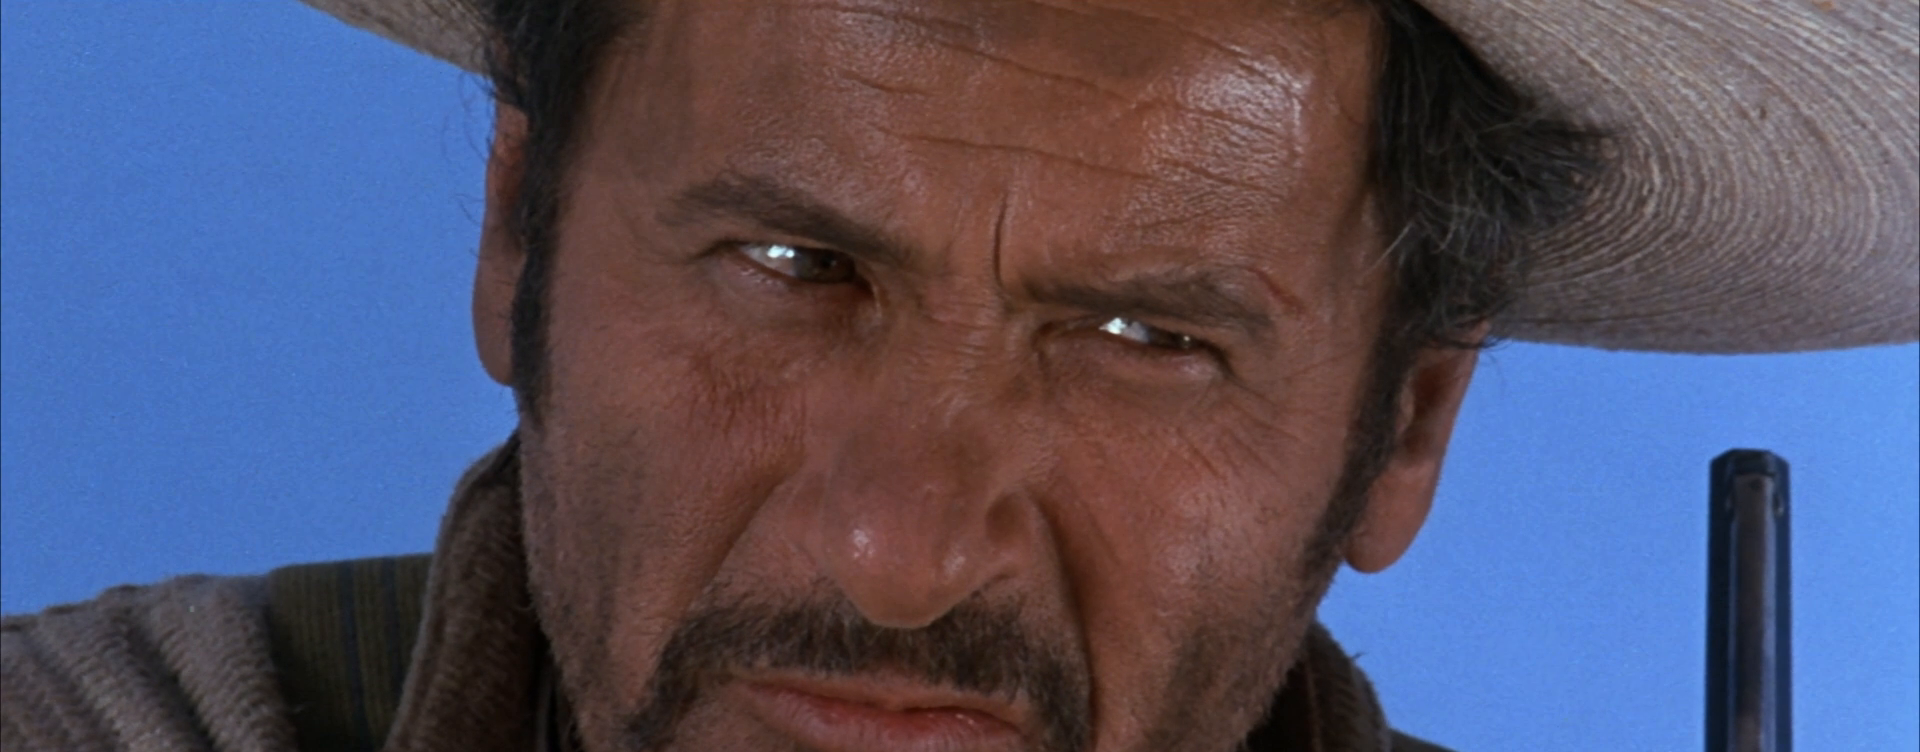
\includegraphics[width=0.7\linewidth]{images/bueno_feo_malo_frame_0131.png}
		\caption{\smaller Original clean frame extracted from a restored 35mm copy of IL BUONO, IL BRUTTO, IL CATTIVO (1966)} 
	\end{figure}
		\begin{figure}[h!]
		\centering
		\fbox{
\includegraphics[width=0.7\linewidth]{images/mask_160.png}}
		\caption{\smaller Artefacts mask generated with the custom library} 
	\end{figure}\\
	The first dataset generated, was just superimposing the black mask to the image. This gave semi-realistic results, but comparing with real damaged frames, it still seemed fake. To improve the performance of the model, and the realism of the dataset \textbf{edge smoothing} has been introduced around the annotated regions. This was achieved by applying a Gaussian blur at the boundaries of the segmented artefacts, thereby mitigating the model's tendency to focus solely on high-contrast transitions.\\
	\begin{figure}[h!]
		\centering
		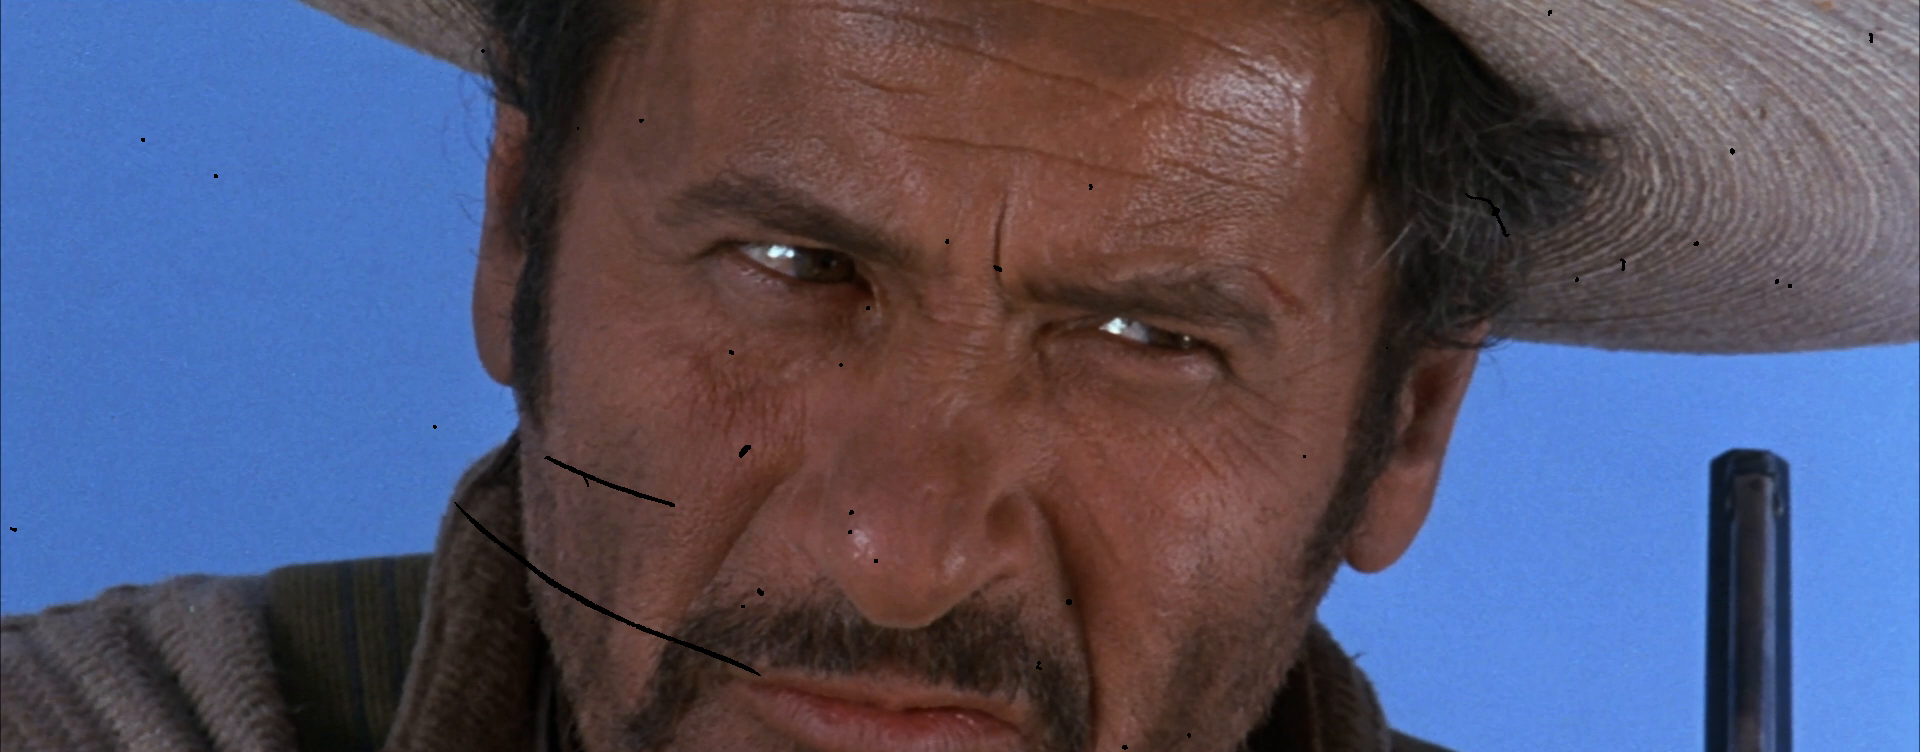
\includegraphics[width=0.7\linewidth]{images/image_binary.png}
		\caption{\smaller Image generated superimposing the mask into the original frame.} 
	\end{figure}
	\begin{figure}[h!]
		\centering
		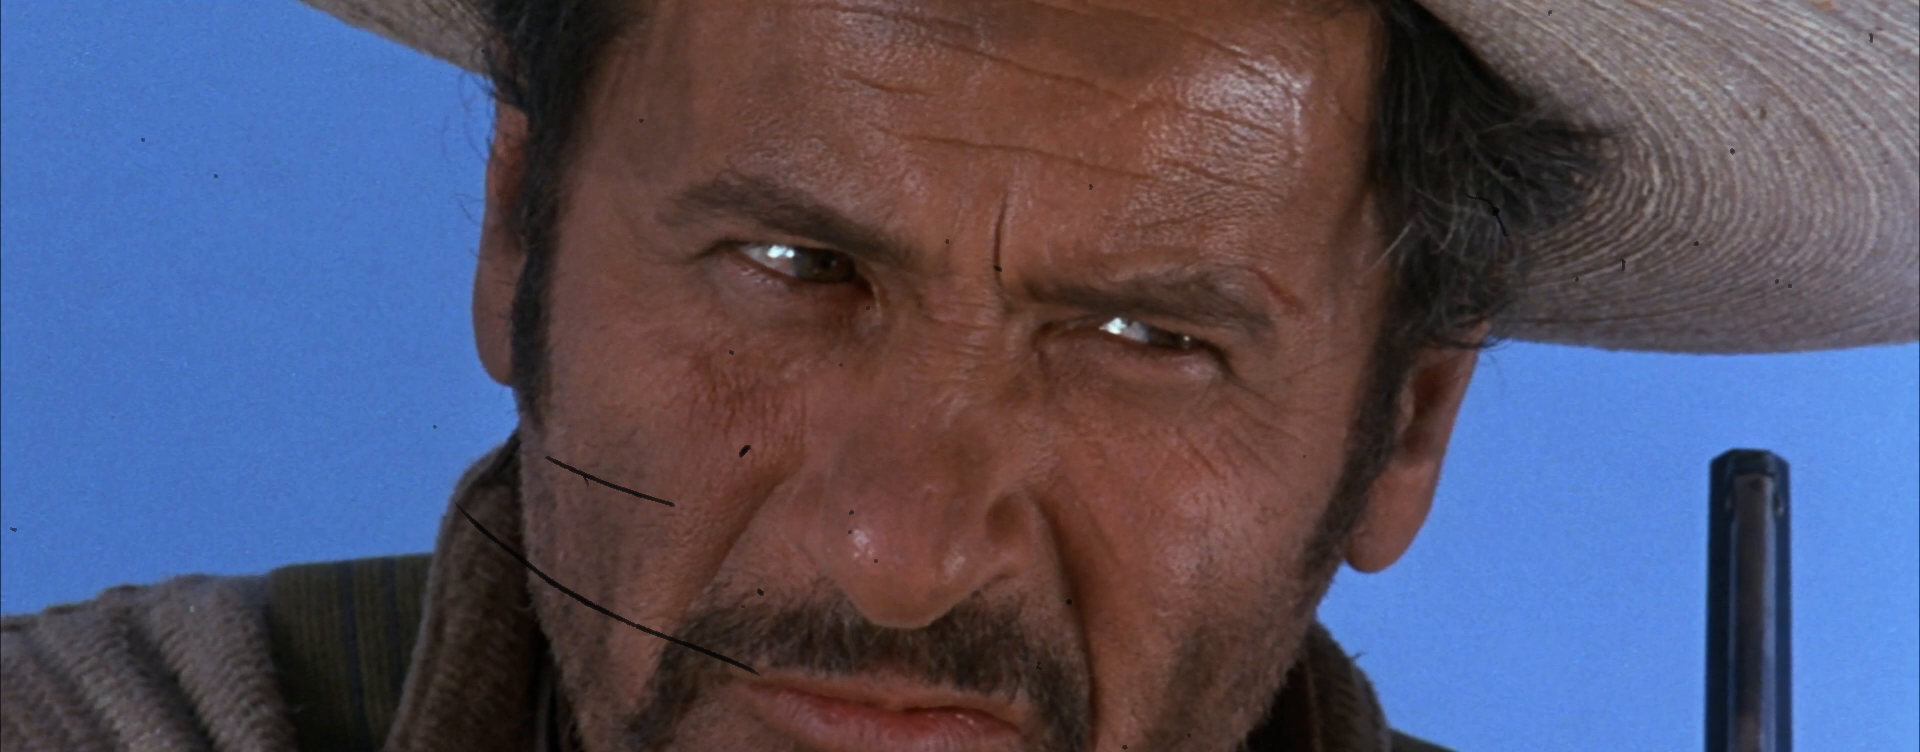
\includegraphics[width=0.7\linewidth]{images/image_blur.png}
		\caption{\smaller Image generated adding gaussian blur around the artefacts in the mask.} 
	\end{figure}\\
	\subsection{Pretraining dataset}
	In order to improve convergence and provide a better initialization for the segmentation model, I also leveraged a separate synthetic dataset provided to me through direct communication with the lead author of the FILM-AA paper. This new dataset—created with the same methodology as my primary synthetic dataset—contains over XXX annotated images. However, instead of being based on restored film transfers, these frames were derived from high-resolution scans of 35mm still images from various (not provided) sources.\\\\
	Although this dataset is not perfectly aligned with the final application domain of degraded motion picture footage, it offers valuable priors on the visual texture and artifact distribution commonly seen in film. As such, it was used for pretraining the segmentation network, which was later fine-tuned on my custom dataset to adapt it to the specific degradation patterns present in cinematic material.
			\begin{figure}[h!]
		\centering
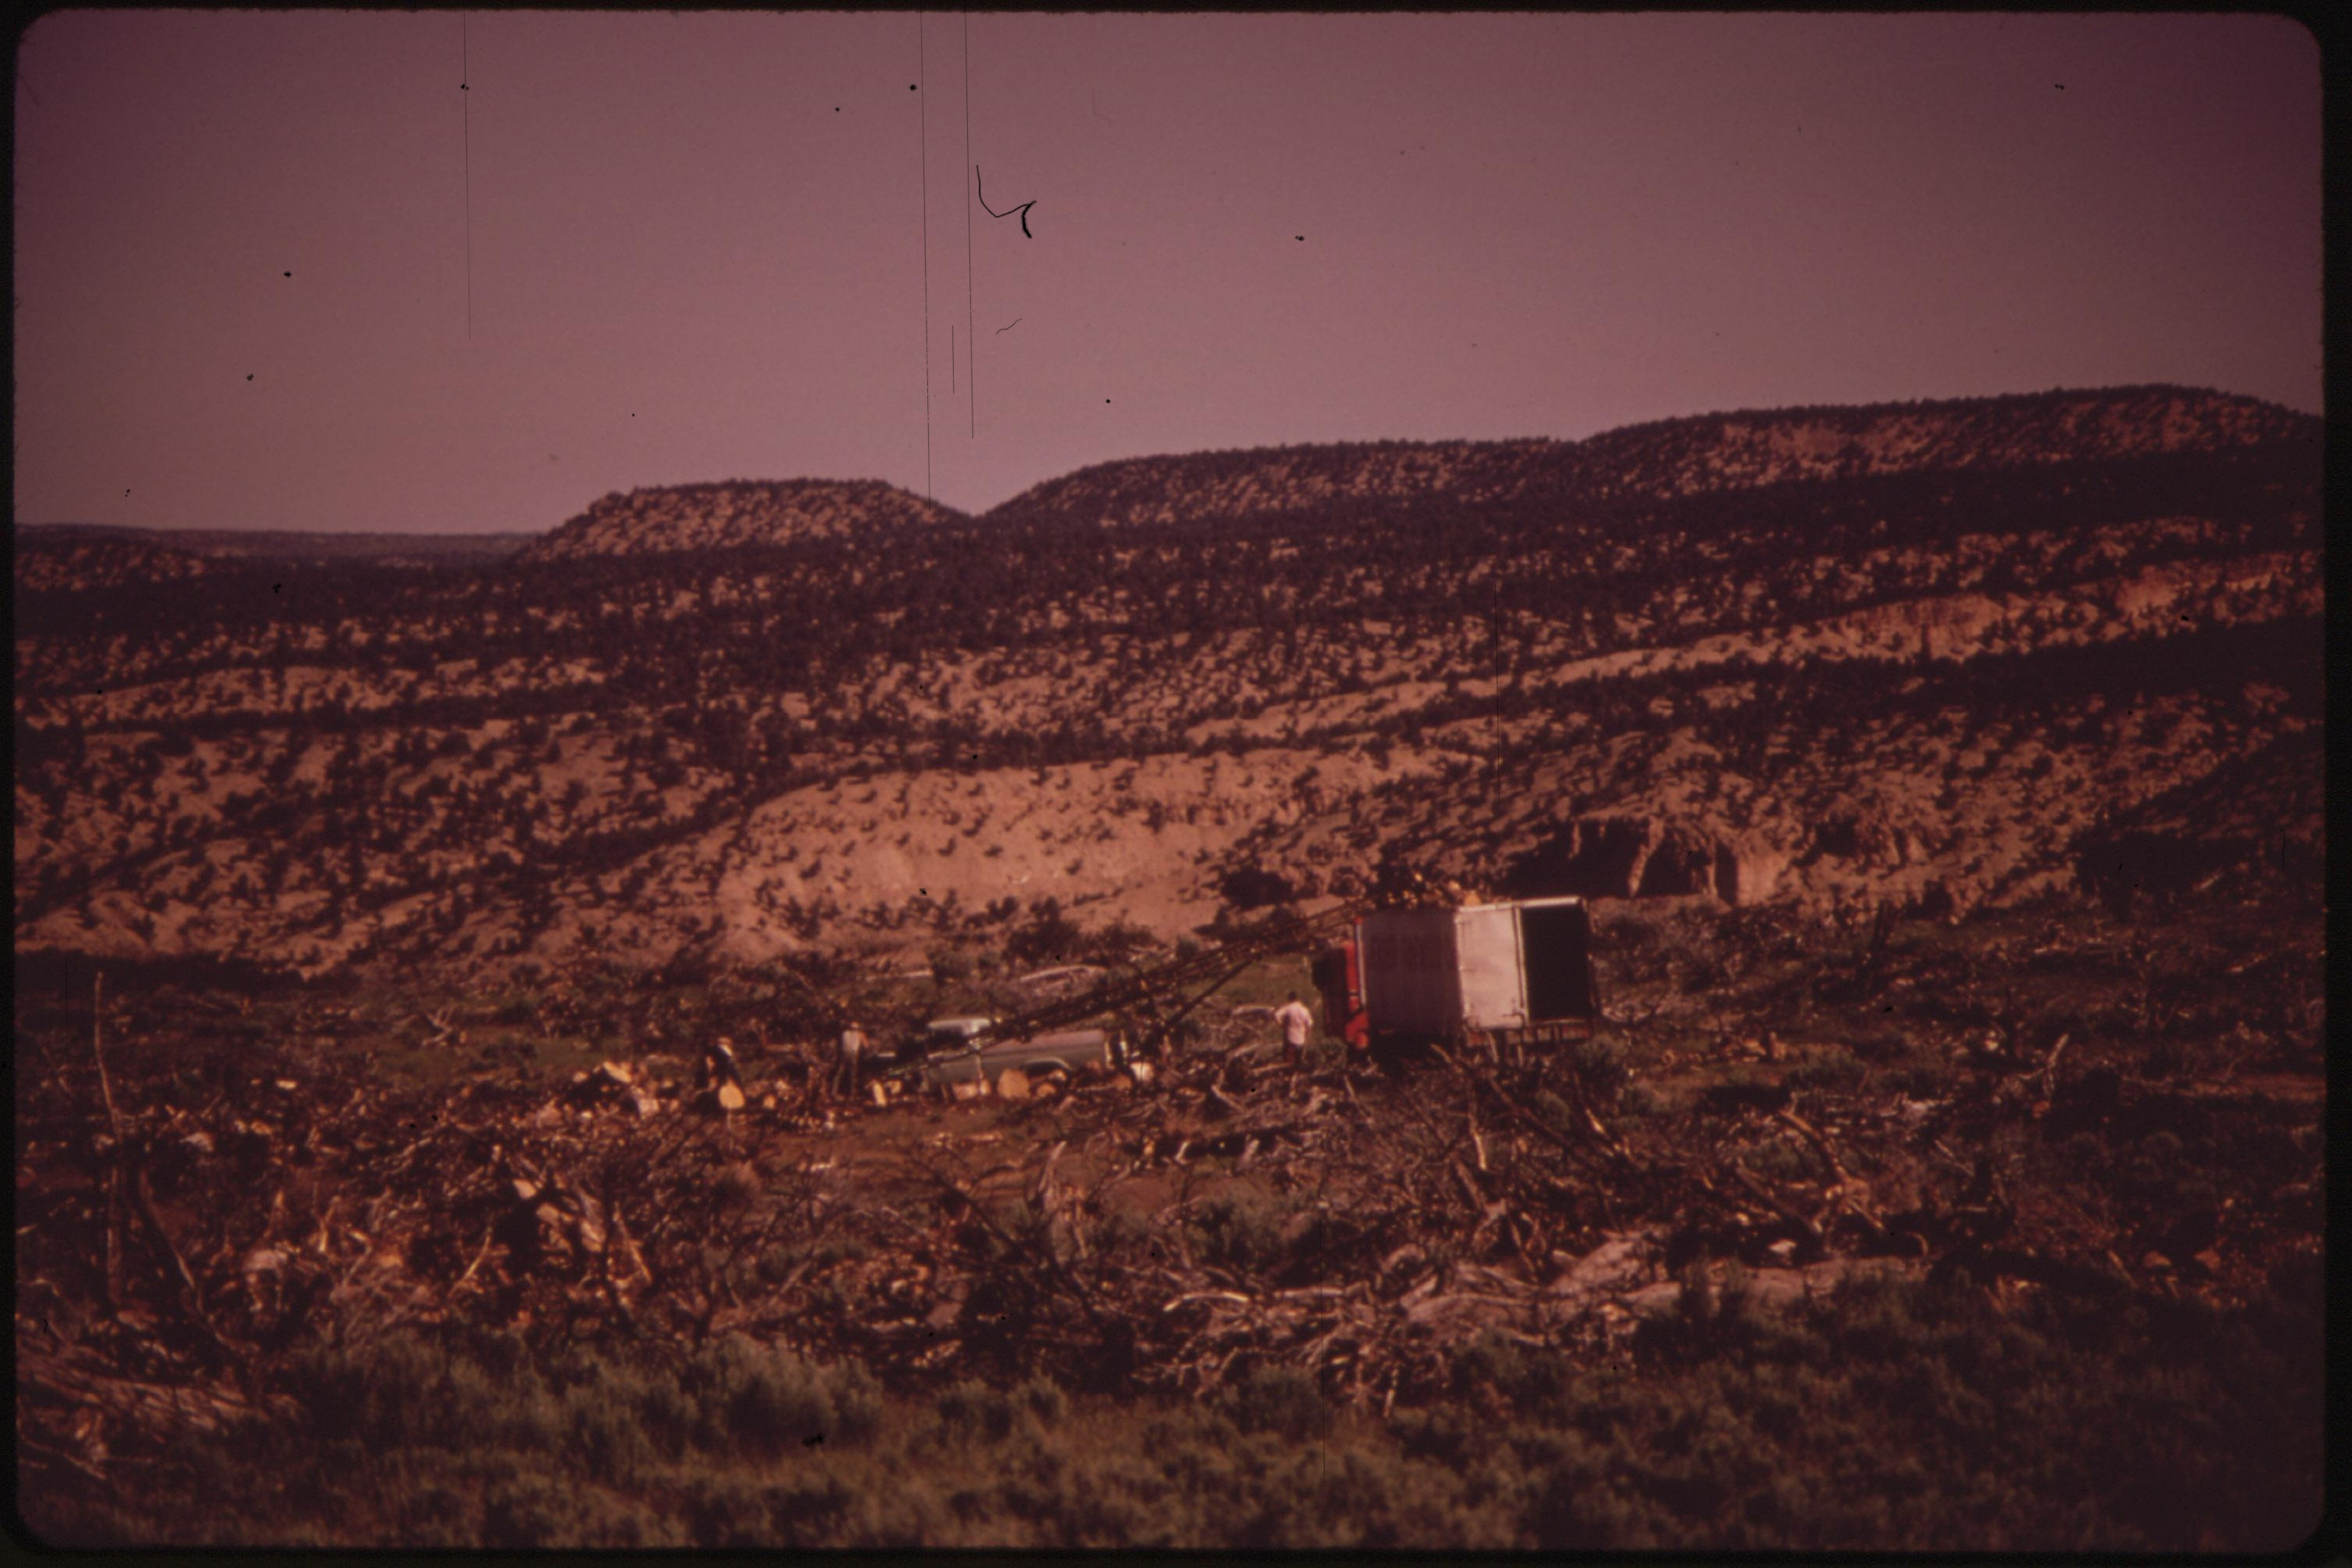
\includegraphics[width=0.5\linewidth]{images/docum.jpg}
		\caption{\smaller Example image of the Documartica dataset} 
	\end{figure}
	
	\subsection{Testing dataset}
	To qualitatively evaluate the performance of the entire restoration pipeline on real-world data, I will use samples from the \textit{Hearst Metrotone News Collection} \cite{newsreel}. This collection, owned by the Regents of the University of California and curated by the UCLA Film \& Television Archive since 1981, comprises a vast archive of historical newsreels originally recorded on 35mm film. The archive contains approximately 25 million feet of 35mm footage and an additional 2 million feet of 16mm film, accompanied by rich contextual documentation.\\\\
	The materials selected for testing have been digitized using a high-resolution, high dynamic range (HDR) film scanner, ensuring the preservation of fine-grained image details and subtle degradations. This allows for a realistic and visually meaningful evaluation of the model's ability to identify and restore artifacts in archival footage.
	\begin{figure}[h!]
		\centering
		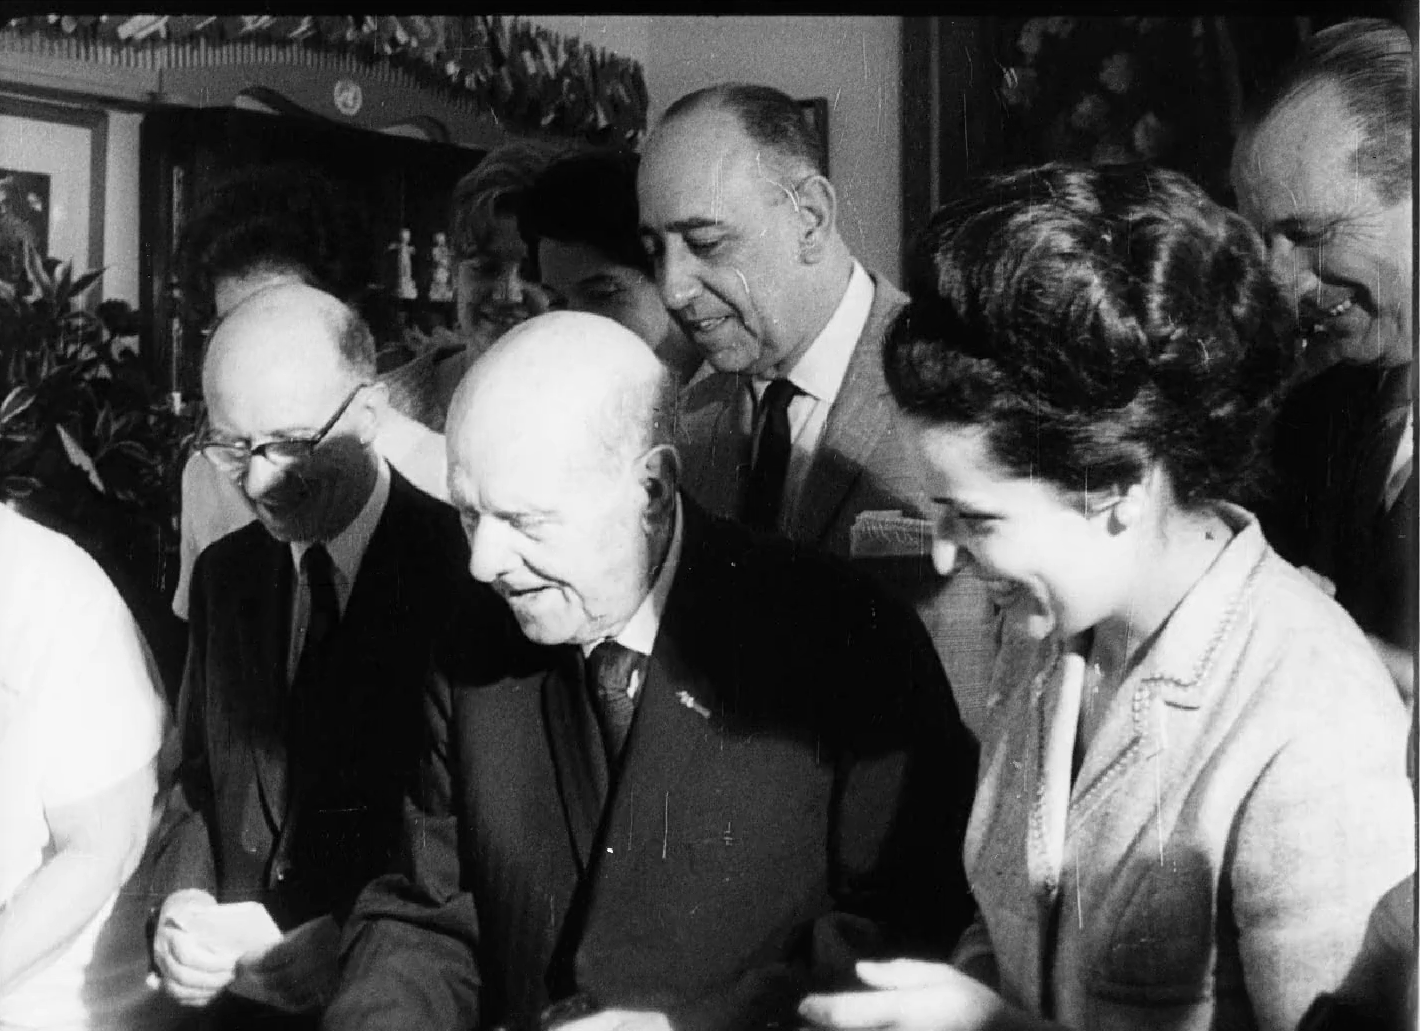
\includegraphics[width=0.5\linewidth]{images/news.png}
		\caption{\smaller Example image of the testing dataset} 
	\end{figure}
	
	\newpage
	\section{Time Schedule}
	\setlength{\arrayrulewidth}{.7 pt}
	\begin{table}[ht!]
		\centering
		\begin{tabular}{|C|D|L|R|}
			\hline
			\textbf{Week} & \textbf{Date} & \textbf{Task Name} & \textbf{Deliverable} \\ \hline
			\rowcolor{green} 1 & 27/01 - 02/02 & Read and research SOTA solutions & - \\ \hline
			\rowcolor{green} 2 & 03/02 - 09/02 & Explore available online datasets (T1) & Dataset \\ \hline
			\rowcolor{yellow} 3 & 10/02 - 16/02 & Implement and create a synthetic dataset (T2) & - \\ \hline
			\rowcolor{green} 4 & 17/02 - 23/02 & Explore segmentation solutions to detect film damage (T3) & - \\ \hline
			\rowcolor{green} 5 & 24/02 - 02/03 & T3 & Initial segmentation model results \\ \hline
			\rowcolor{green} 	6 & 03/03 - 09/03 & Prepare and redact the initial report delivery & Initial Report \\ \hline
			\rowcolor{black}   % Black row with white text
			\multicolumn{2}{|c|}{\textcolor{white}{10/03/2025}} & \multicolumn{2}{c|}{\textcolor{white}{\textbf{DUE INITIAL REPORT}}} \\ \hline
			\rowcolor{green} 7 & 10/03 - 16/03 & Improve the synthetic dataset, T3, T4 & Result comparison \\ \hline
			\rowcolor{green} 8 & 17/03 - 23/03 & Explore inpainting solutions and implement a starting model (T5) & - \\ \hline
			\rowcolor{yellow} 9 & 24/03 - 30/03 & T5 & Initial inpainting model results \\ \hline
			\rowcolor{red} 10 & 31/03 - 06/04 & Develop a solution to incorporate temporal bias into the inpainting diffusion model (T6) & - \\ \hline
			\rowcolor{red}11 & 07/04 - 13/04 & Prepare a dataset to train \textit{T6} model and train the model & Result comparison \\ \hline
			\rowcolor{green} 12 & 14/04 - 20/04 & Prepare and redact Progress Report I & Progress Report I \\ \hline
			\rowcolor{black}   % Black row with white text
			\multicolumn{2}{|c|}{\textcolor{white}{20/04/2025}} & \multicolumn{2}{c|}{\textcolor{white}{\textbf{DUE PROGRESS REPORT I}}} \\ \hline
	13 & 21/04 - 27/04 & Explore different architectures for inpainting restoration (T7), T6 & - \\ \hline
	14 & 28/04 - 04/05 & Train and/or test T7 models & Result comparison \\ \hline
	15 & 05/05 - 11/05 & Prepare models for GUI (T8) & Model inference service \\ \hline
	16 & 12/05 - 18/05 & T7, T8 & Final GUI \\ \hline
	17 & 19/05 - 25/05 & Prepare and redact Progress Report II & Progress Report II \\ \hline
	\rowcolor{black}   % Black row with white text
	\multicolumn{2}{|c|}{\textcolor{white}{25/05/2025}} & \multicolumn{2}{c|}{\textcolor{white}{\textbf{DUE PROGRESS REPORT II}}} \\ \hline
		\end{tabular}
	\end{table}
	
	\begin{table}[ht!]
		\centering
		
		\begin{tabular}{|C|D|L|R|}
					\hline
				\textbf{Week} & \textbf{Date} & \textbf{Task Name} & \textbf{Deliverable} \\ \hline
	18 & 26/05 - 01/06 & Prepare and redact final report proposal & - \\ \hline
	19 & 02/06 - 08/06 & Prepare and redact final report proposal & - \\ \hline
	20 & 09/06 - 15/06 & Prepare and redact final report proposal & Final report proposal \\ \hline
	\rowcolor{black}   % Black row with white text
	\multicolumn{2}{|c|}{\textcolor{white}{15/06/2025}} & \multicolumn{2}{c|}{\textcolor{white}{\textbf{DUE FINAL REPORT PROPOSAL}}} \\ \hline
	21 & 16/06 - 22/06 & Prepare presentation slides & Presentation \\ \hline
	\rowcolor{black}   % Black row with white text
	\multicolumn{2}{|c|}{\textcolor{white}{20/06/2025}} & \multicolumn{2}{c|}{\textcolor{white}{\textbf{DUE PRESENTATION PROPOSAL}}} \\ \hline
	22 & 23/06 - 29/06 & Prepare final dossier & Dossier \\ \hline
	\rowcolor{black}   % Black row with white text
	\multicolumn{2}{|c|}{\textcolor{white}{29/06/2025}} & \multicolumn{2}{c|}{\textcolor{white}{\textbf{DUE FINAL DOSSIER}}} \\ \hline
		\end{tabular}
		\caption{Weekly Planning}
	\end{table}
	\newpage
	\subsection{Review}
In this section, I provide a week-by-week summary of the project's progress, aligned with the scheduled tasks for each period. This overview is meant to give a general sense of the work completed without going into technical or implementation-specific details, which will be covered in the following section. The objective here is to offer a clear and concise account of the project's development over time.\newline \\
	\begin{tabular}{|C|D|L|R|}
		\hline
		\rowcolor{green}
		1 & 27/01 - 02/02 & Read and research SOTA solutions & - \\
		\hline
		\multicolumn{4}{|>{\arraybackslash}m{\linewidth}|}{
			\vspace{1em}
The first week focused on reviewing relevant literature and surveying existing solutions related to the project. The primary outcome was the selection of an initial architecture consisting of two core components: a segmentation model and an inpainting model. Specific implementation details will be discussed in the following section.
			\vspace{1em}
		} \\
		\hline
	\end{tabular}
	\newline
	\vspace{0.3em}
	\newline
	\begin{tabular}{|C|D|L|R|}
	\hline
	\rowcolor{green}
	\rowcolor{green} 2 & 03/02 - 09/02 & Explore available online datasets (T1) & Dataset \\ 
	\hline
	\multicolumn{4}{|>{\arraybackslash}m{\linewidth}|}{
		\vspace{1em}
		The focus this week was identifying a suitable dataset for the task. A general explanation has already been included in the \textit{Initial Report}; for clarity, that explanation remains in this report in {\color{blue}blue} font (\hyperref[sec:Dataset]{{\color{blue}Section 5}}). Additional information is provided in standard text throughout the document. 
		\vspace{1em}
	} \\
	\hline
\end{tabular}
	\newline
\vspace{0.3em}
\newline
\begin{tabular}{|C|D|L|R|}
	\hline
	\rowcolor{yellow} 3 & 10/02 - 16/02 & Implement and create a synthetic dataset (T2) & - \\ \hline
	\multicolumn{4}{|>{\arraybackslash}m{\linewidth}|}{
		\vspace{1em}
This week was dedicated to customizing the FILM-AA library to dynamically generate synthetic datasets using custom images. Additionally, I implemented the necessary classes and functions required to train models using these datasets.
		\vspace{1em}
	} \\
	\hline
\end{tabular}
	\newline
\vspace{0.3em}
\newline
\begin{tabular}{|C|D|L|R|}
	\hline
\rowcolor{green} 4 & 17/02 - 23/02 & Explore segmentation solutions to detect film damage (T3) & - \\ \hline
	\multicolumn{4}{|>{\arraybackslash}m{\linewidth}|}{
		\vspace{1em}
This week focused on identifying a suitable segmentation architecture. After reviewing several papers, I selected U-Net as the baseline model. Although transformer-based segmentation models were considered, they were ultimately discarded. The U-Net implementation was adapted to fit the project’s requirements and to simplify training. Code details are documented in the source code via comments and in the \textit{README.md} file of the repository. 
		\vspace{1em}
	} \\
	\hline
\end{tabular}
\newline
\vspace{0.3em}
\newline
\begin{tabular}{|C|D|L|R|}
	\hline
	\rowcolor{green} 5 & 24/02 - 02/03 & T3 & Initial segmentation model results \\ \hline
	\multicolumn{4}{|>{\arraybackslash}m{\linewidth}|}{
		\vspace{1em}
This week continued the work on segmentation. The previously chosen U-Net model was finalized and adapted further. Again, implementation details are documented within the code and in the repository’s \textit{README.md}. 
		\vspace{1em}
	} \\
	\hline
\end{tabular}
\newline
\vspace{0.3em}
\newline
\begin{tabular}{|C|D|L|R|}
	\hline
\rowcolor{green} 7 & 10/03 - 16/03 & Improve the synthetic dataset, T3, T4 & Result comparison \\ \hline
	\multicolumn{4}{|>{\arraybackslash}m{\linewidth}|}{
		\vspace{1em}
Although improvements to the synthetic dataset were planned for this week, much of this work had already been completed during earlier training sessions with the U-Net. This week primarily involved preparing an inference workflow to facilitate the comparison of results across different trained models. Detailed evaluations are presented in the development section. 
		\vspace{1em}
	} \\
	\hline
\end{tabular}
\newline
\vspace{0.3em}
\newline
\begin{tabular}{|C|D|L|R|}
	\hline
	\rowcolor{green} 8 & 17/03 - 23/03 & Explore inpainting solutions and implement a starting model (T5) & - \\ \hline
	\multicolumn{4}{|>{\arraybackslash}m{\linewidth}|}{
		\vspace{1em}
This week was dedicated to researching diffusion-based inpainting frameworks. I ultimately selected RePaint, as detailed in the State of the Art section. Parallel to this, I continued testing ways to improve the U-Net segmentation models.  
		\vspace{1em}
	} \\
	\hline
\end{tabular}
\newline
\vspace{0.3em}
\newline
\begin{tabular}{|C|D|L|R|}
	\hline
	\rowcolor{yellow} 9 & 24/03 - 30/03 & T5 & Initial inpainting model results \\ \hline	\multicolumn{4}{|>{\arraybackslash}m{\linewidth}|}{
		\vspace{1em}
While this week was intended to yield initial results from the inpainting model, most of the time was spent adapting the RePaint implementation, constructing a test dataset, and continuing with pretraining experiments from the previous week. As a result, the planned work extended into the following week.
		\vspace{1em}
	} \\
	\hline
\end{tabular}
\newline
\vspace{0.3em}
\newline
\begin{tabular}{|C|D|L|R|}
	\hline
	\rowcolor{red} 10 & 31/03 - 06/04 & Develop a solution to incorporate temporal bias into the inpainting diffusion model (T6) & - \\ \hline
	\rowcolor{red}11 & 07/04 - 13/04 & Prepare a dataset to train \textit{T6} model and train the model & Result comparison \\ \hline	\multicolumn{4}{|>{\arraybackslash}m{\linewidth}|}{
		\vspace{1em}
Unfortunately, I was unable to complete the tasks for these weeks as planned. Week 10 was spent performing test runs with the RePaint model. By week 11, I had achieved end-to-end results for the full pipeline. These outcomes are discussed later in this report. 
		\vspace{1em}
	} \\
	\hline
\end{tabular}
	\section{Development}
	\subsection{Pipeline}
	Before entering into model implementation, code development and preliminary results, it is essential to establish a clear architectural framework that will guide this project. Given the complexity of film restoration, particularly when working with analog formats such as 35mm film, the architecture must accound for both the visual characteristics of film and the nature of degradations we aim to correct.\\
	To this end, the proposed pipeline is composed of two main stages: segmentation and restoration. First, a U-Net-based segmentator identifies and isolates regions of damage such as dust, scratches and other artifacts. This damage mask is then passed as input to a diffusion-based inpainting model, which reconstructs the missing or corrupted regions while preserving the original film's texture, tone and grain.\\
	This two-step approach allows for more targeted restorations, as the inpainting model can focus solely on the areas marked as damaged, reducing the risk of altering intact portions of the image. Furthermore, the architecture is designed to incorporate temporal information from adjacent frames, helping ensure consistency and coherence across time; Although this has not yet been implemented, it is one of the objectives for the following weeks. By explicitly separating damage detection from content restoration, the architecture remains modular and interpretable, paving the way for further improvements and extensions. 
	 
	\subsection{Segmentation}
	This section outlines the different stages of experimentation, from initial baselines to advanced pretraining strategies,encompassing architectural experimentation, dataset enhancement, and strategic training techniques. The process is structured into several phases, described below.
	\subsubsection*{Baseline Architectures}
	The initial experimentation involved evaluating a series of established segmentation architectures:
	\begin{itemize}
		\item The original U-Net architecture ~\cite{ronneberger_u-net_2015}
		\item The Attention U-Net (AttU-Net) ~\cite{oktay_attention_2018}
		\item The Recurrent Residual U-Net (R2U-Net) and R2AttU-Net ~\cite{alom_recurrent_2018}
	\end{itemize}
	These models were trained from scratch on a synthetic dataset consisting of 600 images, created during Week 5. As anticipated, the results were suboptimal, primarily due to the limited size of the dataset. One of the main problems all these current model have is having a tendency to detect high-contrast transitions as artefacts.
	\subsubsection*{Dataset Expansion and Preprocessing Enhancements}
	To address the limitations posed by data scarcity, a new dataset of 3000 synthetic artefacts masks was generated. This expansion significantly improved model performance. in addition, the dataset was further refined by introducing \textbf{edge smoothing} around the annotated regions. This was achieved by applying a Gaussian blur at the boundaries of the segmented artefacts, thereby mitigating the model's tendency to focus solely on high-contrast transitions.\\
	\\
	Despite these improvements, the models still exhibited limited generalization capability. One of the hypothesis for these lack of performance was thought to be due to the randomly initialized weights. In the next section this problem will be tackled.
	\subsubsection*{Pretraining Approaches}
	To enhance both convergence speed and final model performance, a series of pretraining strategies were explored:
	\begin{itemize}
		\item \textbf{Denoising Pretraining~\cite{9857234}:} \\
		A denoising task was employed as a proxy pretraining objective using approximately 10,000 images. This allowed the model to learn useful low-level features prior to fine-tuning on the segmentation task. Initial experiments with the U-Net architecture showed clear qualitative improvements in segmentation results.
		\item \textbf{Transfer of Pretraining Across Architectures:}
		Upon validating the benefits of denoising pretraining with the U-Net, the same prodecure was extended to AttU-Net, R2U-Nett and R2AttU-Net. All architectures demonstrated improved performance when initialized with pretrained weights.
		\item \textbf{Multi-Stage Pretraining:}
		In a subsequent refinement, the models were additionally pretrained on the \textbf{Documartica dataset}, a corpus generated similarly to the target dataset but lacking task-specific structures (mainly the frames not being from 35mm scanned films). This intermediate step further improved the model's repesentational capacity. Final fine-tuning was performed using the custom dataset of 3000 images. 
	\end{itemize}
	\subsubsection*{Model Simplification for Computational Efficiency}
	To optimize computational efficiency, the number of channels in all layers of the network was reduced by half. This modification led to a significant reduction in training time without compromising the segmentation quality, as evaluated qualitatively.
	
	\subsubsection*{Final Configuration and Observations}
	The best qualitative performance was achieved using the \textbf{Attention U-Net} architecture, following the full pipeline:
	\begin{enumerate}
		\item Denoising pretraining
		\item Intermediate pretraining on the Documartica Dataset
		\item Final fine-tuning on the task-specific dataset
		\item Reduced-channel model configuration
	\end{enumerate}
	While formal quantitative metrics are not yet available, the observed improvements where consistent across visual inspections. The implementation of a quantitative evaluation protocol is a key objective for the second phase of this project.
	\subsection{InPainting with RePaint}
	RePaint ~\cite{lugmayr2022repaintinpaintingusingdenoising} is an inpainting method based on diffusion models that extends the standard denoising diffusion probabilistic models (DDPMs) by introducing a novel sampling strategy. Specifically, it employs a "repainting schedule"—a combination of reverse and forward diffusion steps—to iteratively refine the content generated within masked regions. This process allows RePaint to more effectively reconstruct complex or irregular missing areas compared to traditional single-pass diffusion-based approaches.\\
	\\
	In the initial phase of this project, the official RePaint repository was cloned for experimental use. As RePaint only provides an inference framework, a pretrained Stable Diffusion model—trained on a dataset referred to here as DATASET—was integrated for performing the inpainting tasks. The primary goal was to assess how well a general-purpose diffusion model could handle restoration on artificially degraded film frames.\\
	\\
	To this end, a set of degraded images was generated, along with corresponding binary masks indicating the corrupted regions. These masks were used directly in the inpainting process, rather than relying on a predicted mask, in this case from the U-Net, to isolate the performance of the inpainting model itself.\\
	\\
	Initial experiments revealed that the model struggled to convincingly restore the masked regions, especially when these were large or structurally complex. To address this, a simple morphological operation—dilation—was applied to the binary masks, expanding the masked areas by a few pixels. This modification helped reduce edge artifacts and led to more coherent results around the boundaries. While this significantly improved performance and yielded results that exceeded initial expectations, the model still faced limitations with larger degraded regions, where the reconstructions often lacked structural and semantic consistency.\\
	\\
	These observations have shaped the direction for the second phase of the project. The next step involves training a custom diffusion model tailored specifically for film restoration tasks. A key enhancement will be the inclusion of temporal conditioning: the model will be conditioned on adjacent frames from the same film sequence. By incorporating visual context from neighboring frames, the model will be better equipped to produce temporally consistent and contextually accurate inpainting results, particularly in scenes with extensive damage or missing data.
	
	
	\section{Preliminar Results}
	As previously stated in this report, a suitable metric for evaluating both the segmentation and inpainting models has yet to be identified. I anticipate completing a comprehensive evaluation study by the time the next report is due. In the meantime, since the models have already been trained, I have compiled a set of inference results to enable a qualitative comparison. 
	\subsection{Segmentation experiments}
	In order to qualitatively assess the performance of the segmentation model, I present several inference examples below. Each result is visualized by overlaying a color-coded mask onto the original frame. The colors represent the following cases:
	
	\begin{itemize} \item \textbf{Yellow:} True Positive (Correct detection of an artifact) \item \textbf{Green:} False Positive (Incorrect detection where no artifact is present) \item \textbf{Red:} False Negative (Missed detection of an existing artifact) \end{itemize}
	
	For clarity, Table~\ref{tab:legend} summarizes the color legend used in the visualizations:
	
\begin{table}[h]
	\centering
	\begin{tabular}{|c|c|c|}
		\hline
		\textbf{Color} & \textbf{Meaning} & \textbf{Interpretation} \\
		\hline
		\textcolor{groc}{Yellow} & True Positive & Correctly detected artifact \\
		\hline
		\textcolor{verd}{Green} & False Positive & Detected artifact where there is none \\
		\hline
		\textcolor{vermell}{Red} & False Negative & Missed artifact \\
		\hline
	\end{tabular}
	\caption{Color legend for segmentation results}
	\label{tab:legend}
\end{table}
The following subsections detail the results according to the different model settings:
\subsubsection*{Reference Image}
For the purposes of this report, I will focus the qualitative comparison on two representative images. These two have been selected due to their problematic nature prone to false positives. While this report highlights only these two images for clarity and space considerations, it is important to note that a more extensive internal evaluation has been conducted across a wider range of examples to verify the generality of the observations presented here.\\
\\
The two selected images serve to illustrate how the models behave across varying difficulty levels and will be consistently used throughout the following comparisons.
	\begin{figure}[h!]
	\centering
	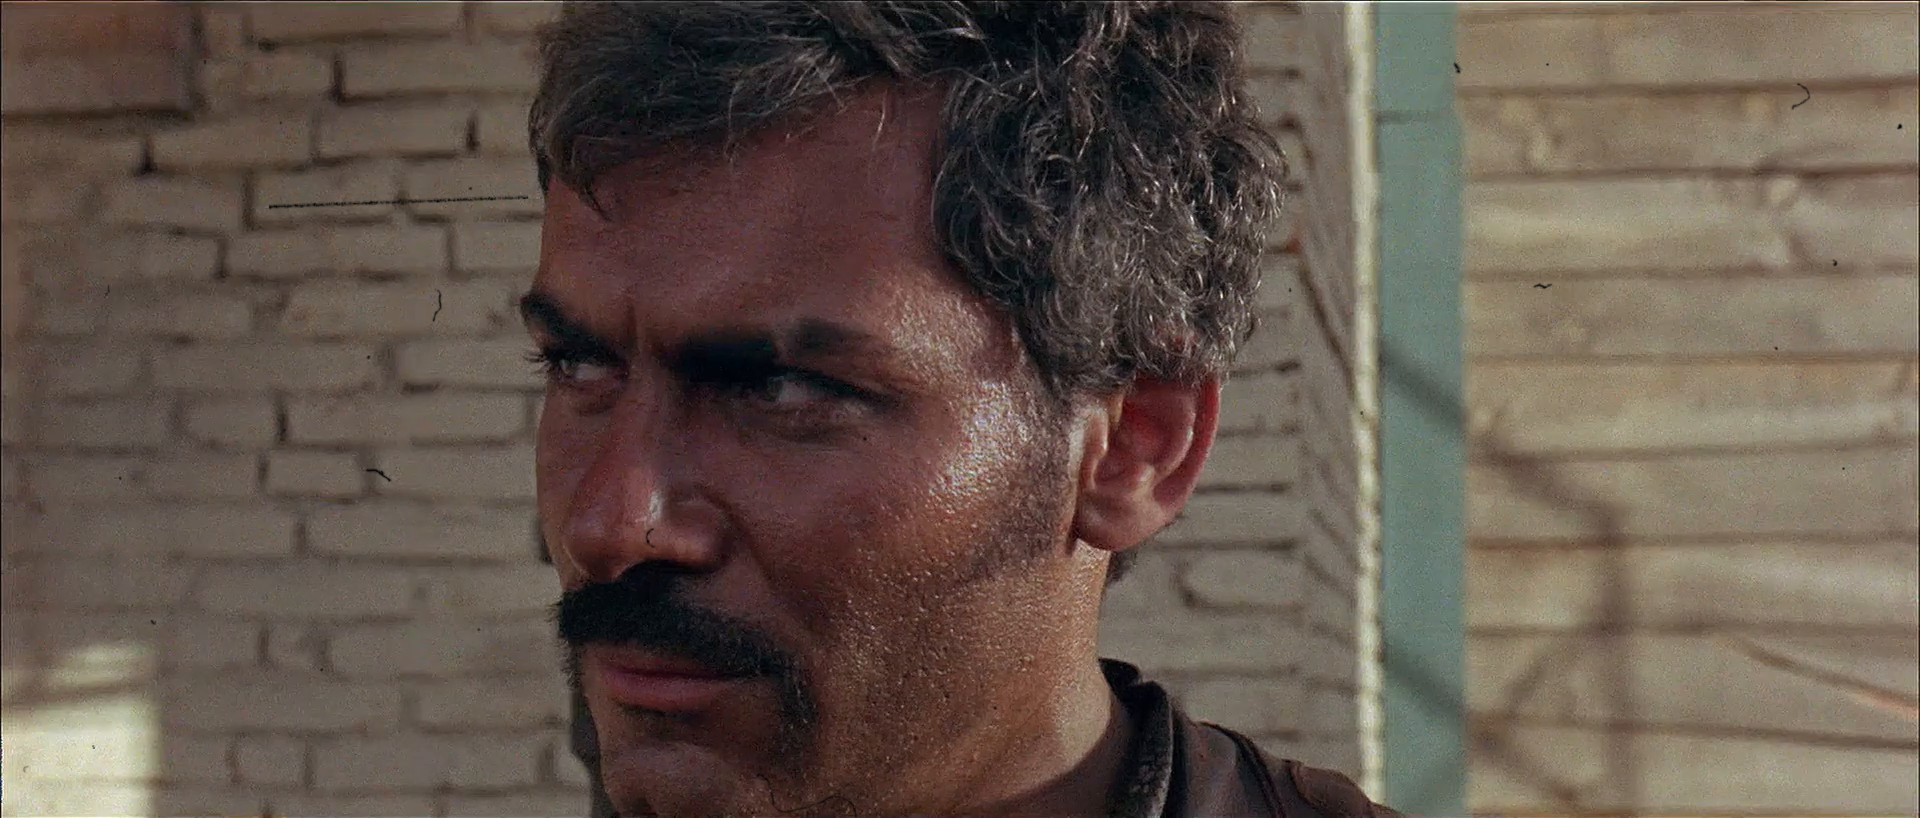
\includegraphics[width=0.8\linewidth]{images/punado_dollars_frame_0084.png}
	\caption{\smaller Test image used in inference. Extracted from the movie A Fistful of Dollars, Sergio Leone 1964, with added synthetic damage.} 
\end{figure}
	\begin{figure}[h!]
	\centering
	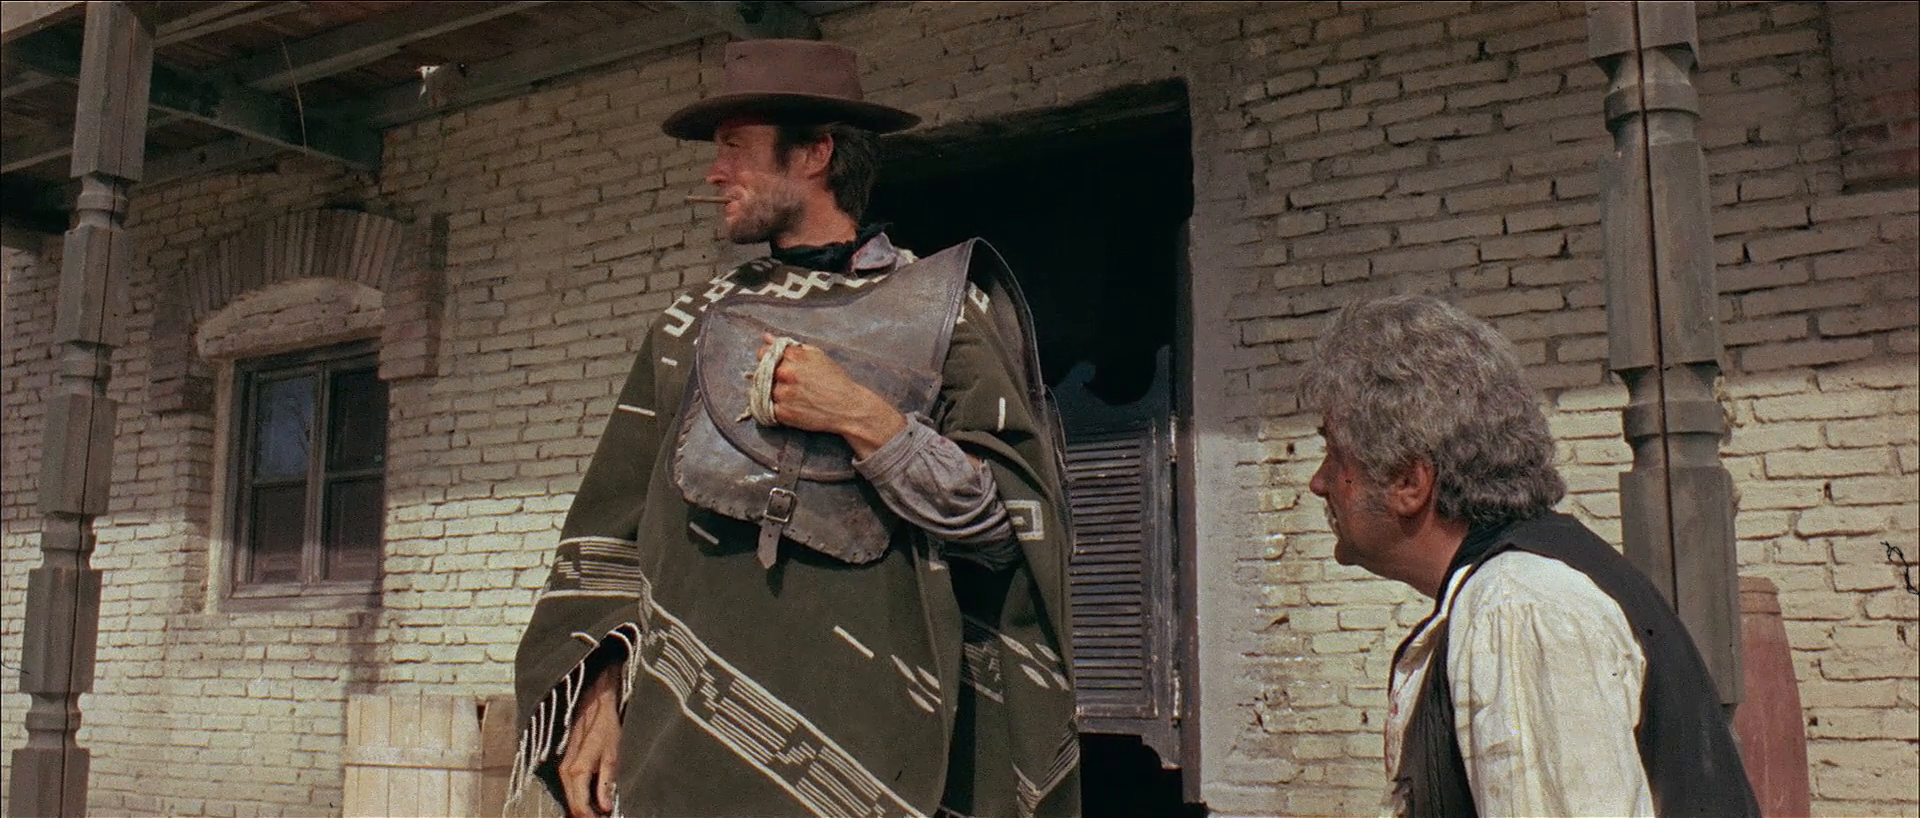
\includegraphics[width=0.8\linewidth]{images/punado_dollars_frame_0122.png}
	\caption{\smaller Test image used in inference. Also extracted from the movie A Fistful of Dollars, Sergio Leone 1964, with added synthetic damage.} 
\end{figure}
\newpage
\subsubsection*{Baseline Model}
First, I present the results obtained using the baseline U-Net model trained on the original dataset:
\begin{figure}[h!]
\centering
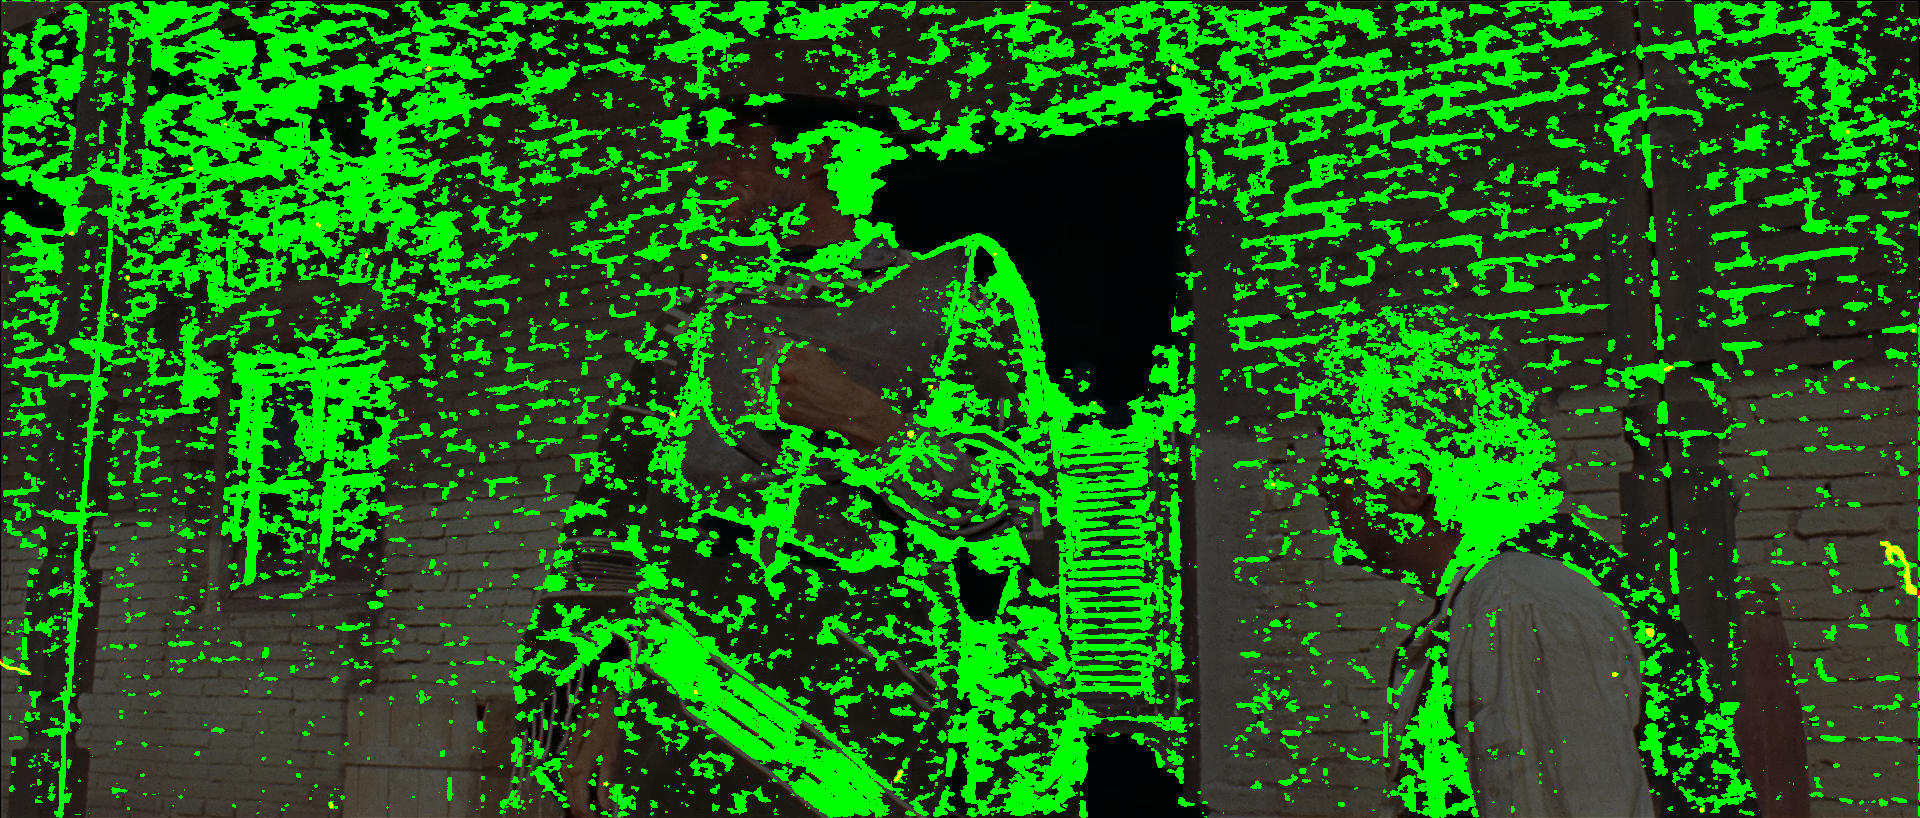
\includegraphics[width=0.7\linewidth]{images/punado_dollars_frame_0122.png_mask_30_epochs_unet_28.png_comparaison.png}
\caption{\smaller Inference result with the Fig. 8 image, using the baseline U-Net model.} 
\end{figure}
\begin{figure}[h!]
	\centering
	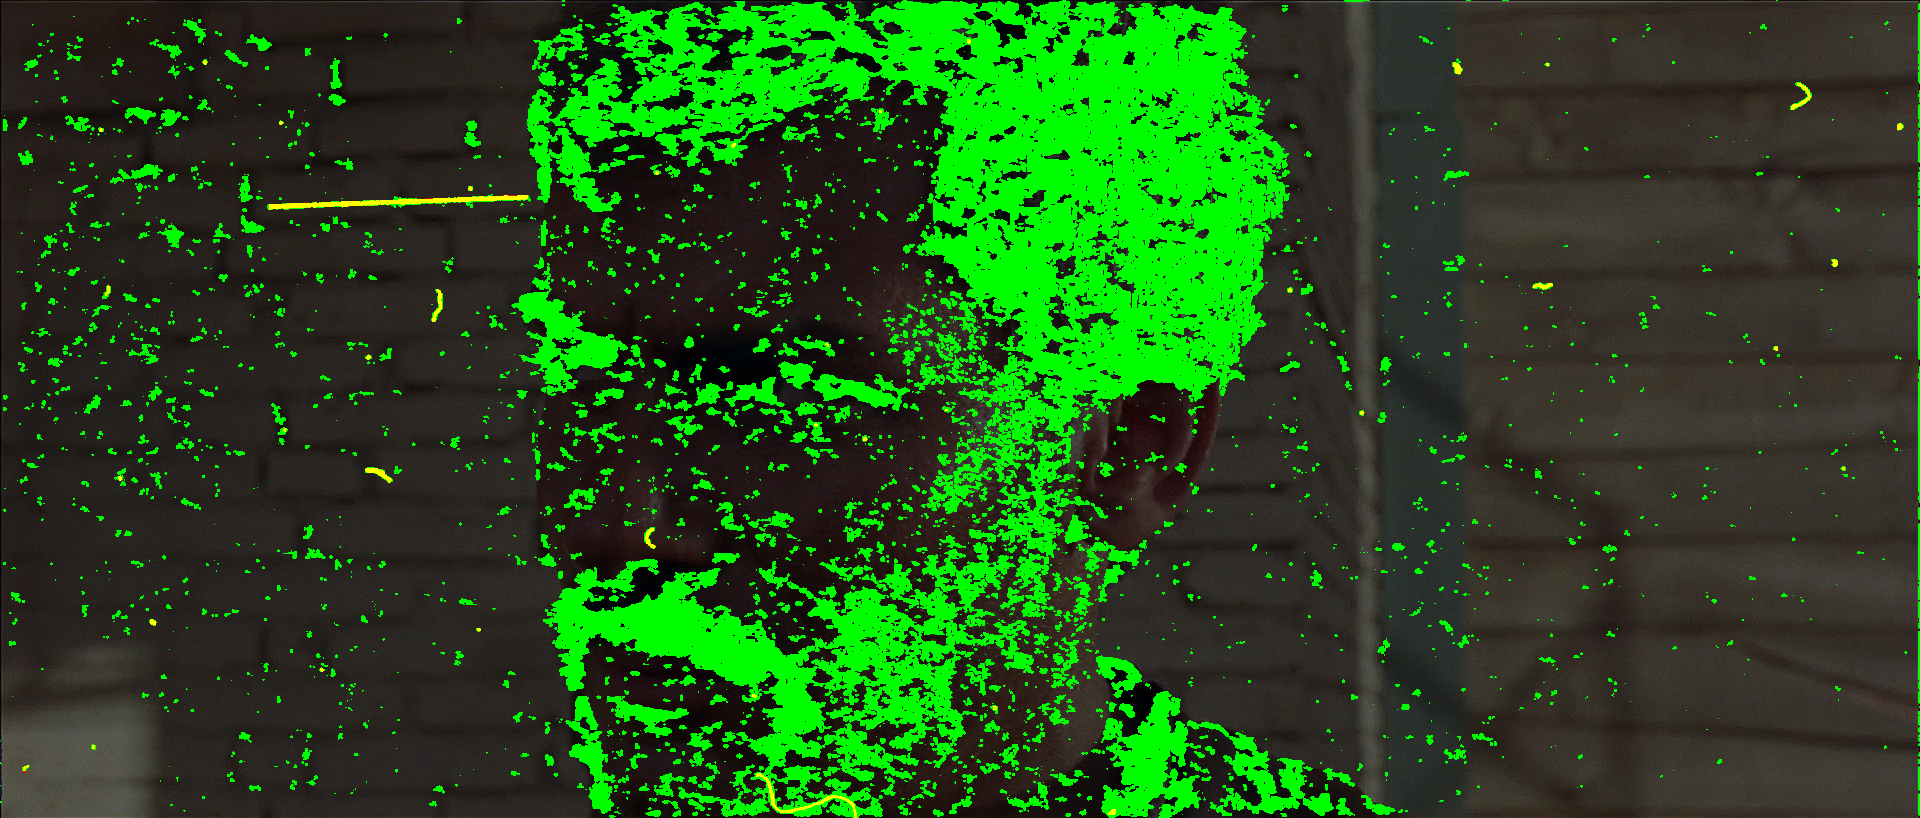
\includegraphics[width=0.7\linewidth]{images/punado_dollars_frame_0084.png_mask_30_epochs_unet_25.png_comparaison.png}
	\caption{\smaller Inference result with the Fig. 7 image, using the baseline U-Net model.} 
\end{figure}
As it can be seened in the image, the model predicts half of the pixels of the image as artefacts. This was attributed to a bad dataset, since the artifacts are just black spots, so the model learns to detect contrast differences and select that. 
\newpage
\subsubsection*{Dataset improvements and new models}
After the poor results of the baseline model+baseline dataset, a new dataset was created. Then it was applied not only to a U-Net, but also an AttU-Net and R2AttU-Net. The following images are the result of the first image tested with the U-Net model to compare.\\
\begin{figure}[h!]
	\centering
	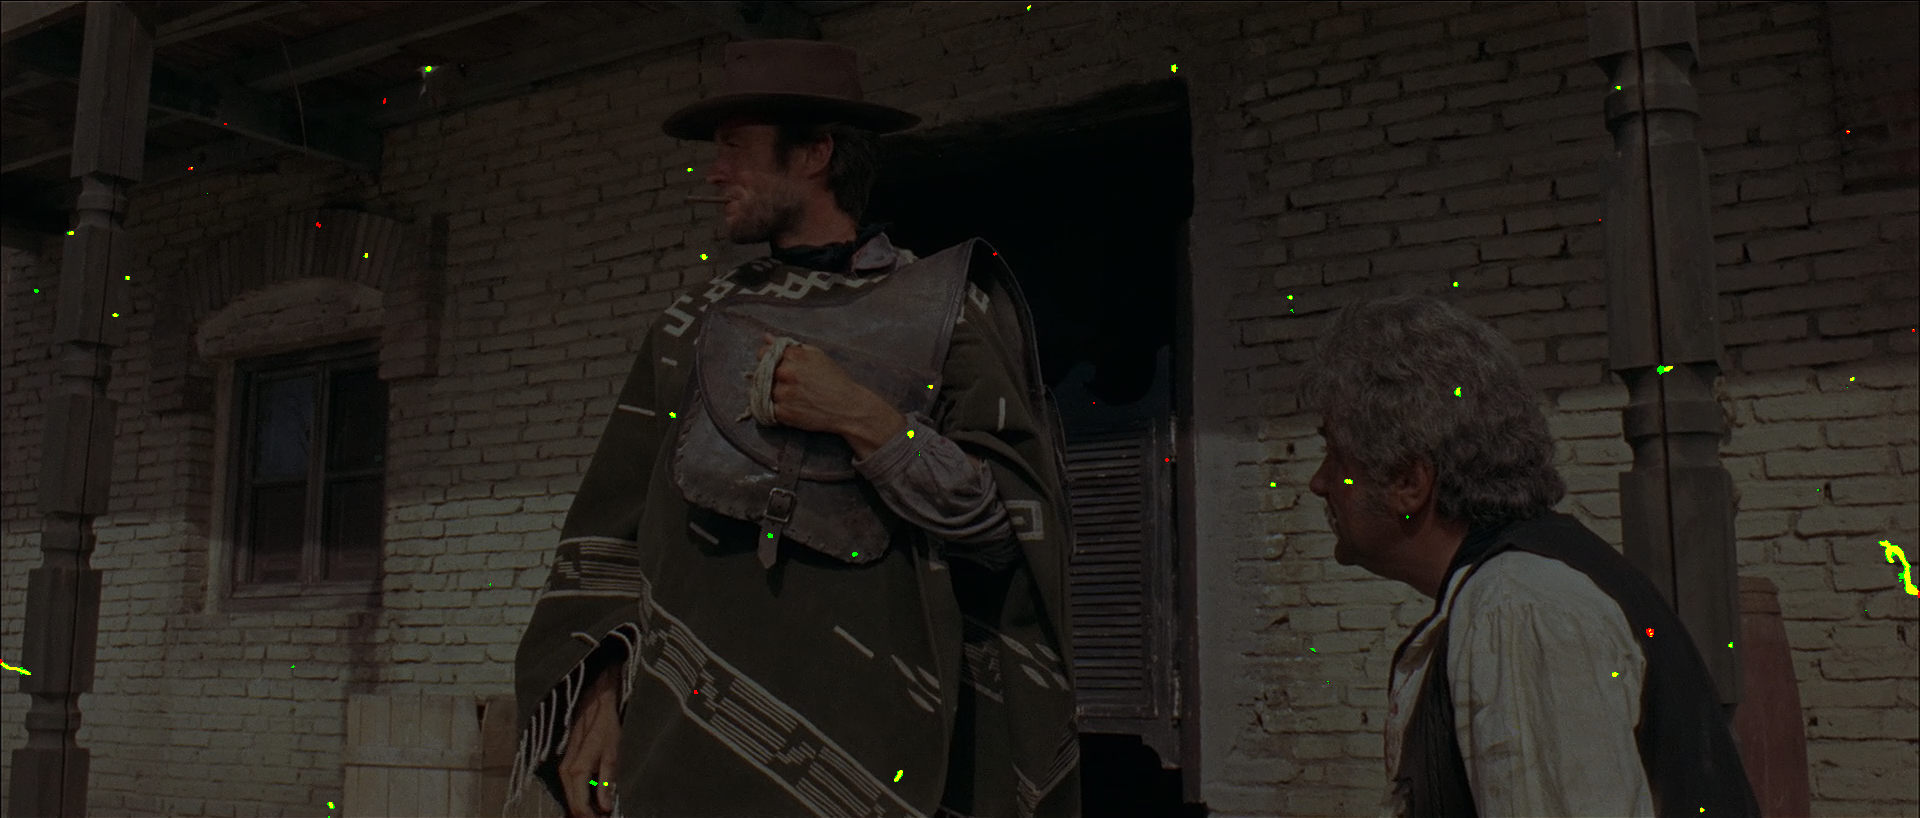
\includegraphics[width=0.7\linewidth]{images/punado_dollars_frame_0122-mask_big_dataset_unet_50_v1.png_comparaison.png}
	\caption{\smaller Inference result with the Fig. 8 image, using the baseline U-Net model with the new perfected dataset.} 
\end{figure}
\begin{figure}[h!]
	\centering
	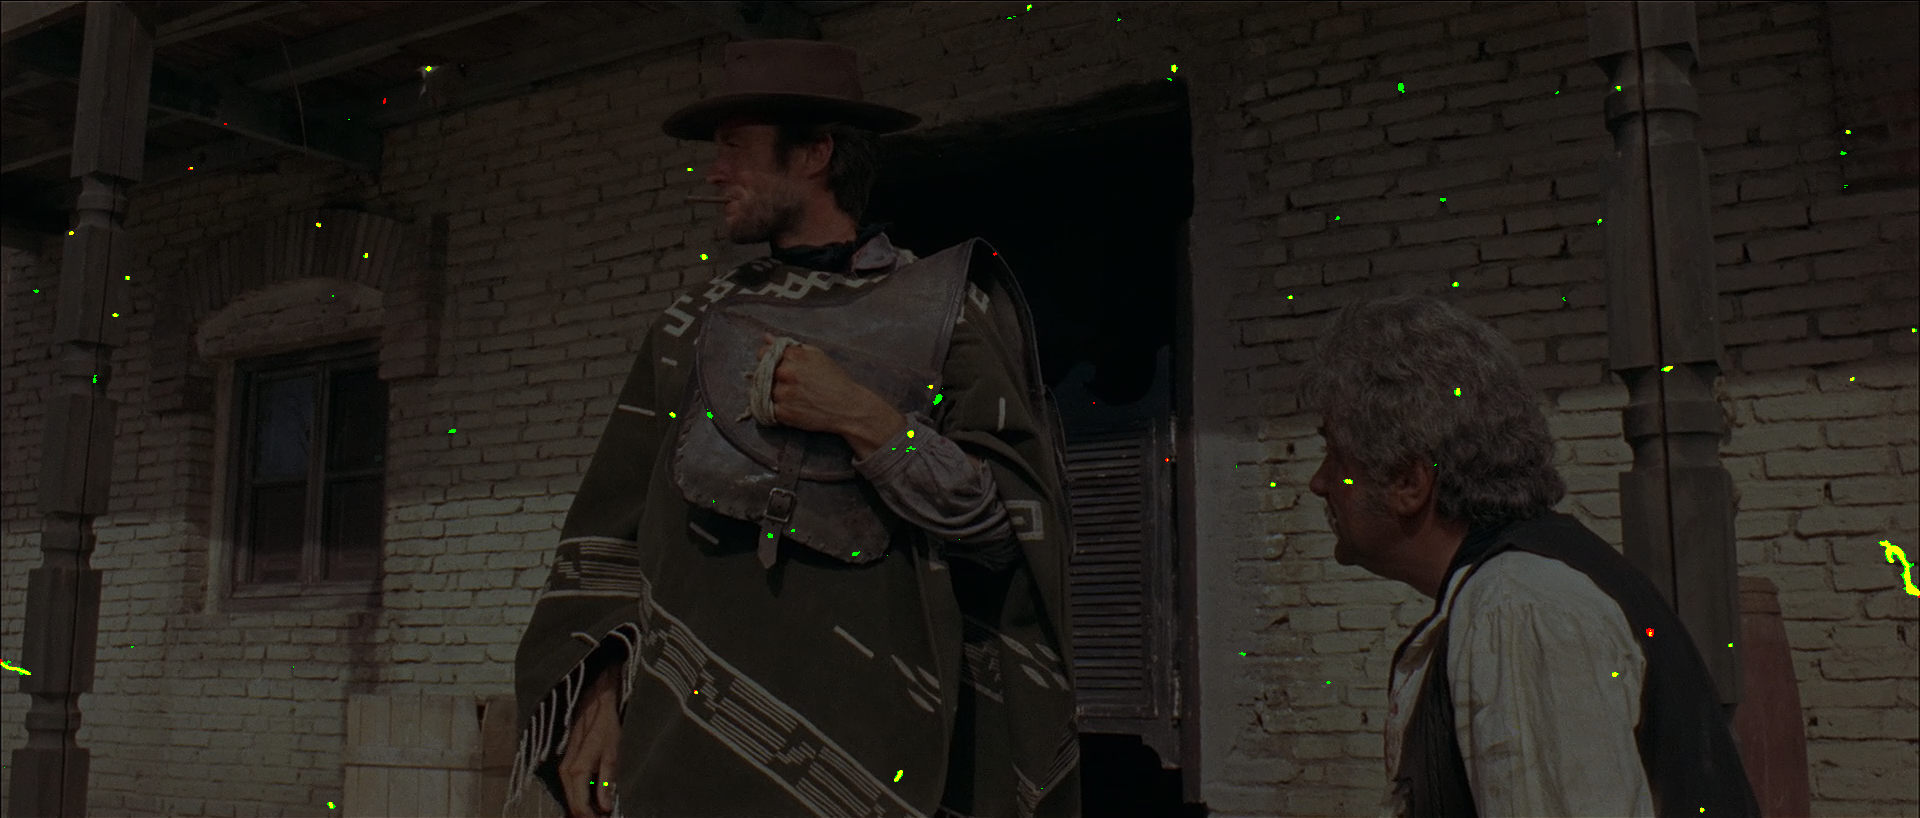
\includegraphics[width=0.7\linewidth]{images/punado_dollars_frame_0122-mask_big_dataset_attunet_40_v1.png_comparaison.png}
	\caption{\smaller Inference result with the Fig. 8 image, using the baseline AttU-Net model with the new perfected dataset.} 
	\label{fig:11}
\end{figure}
\begin{figure}[h!]
	\centering
	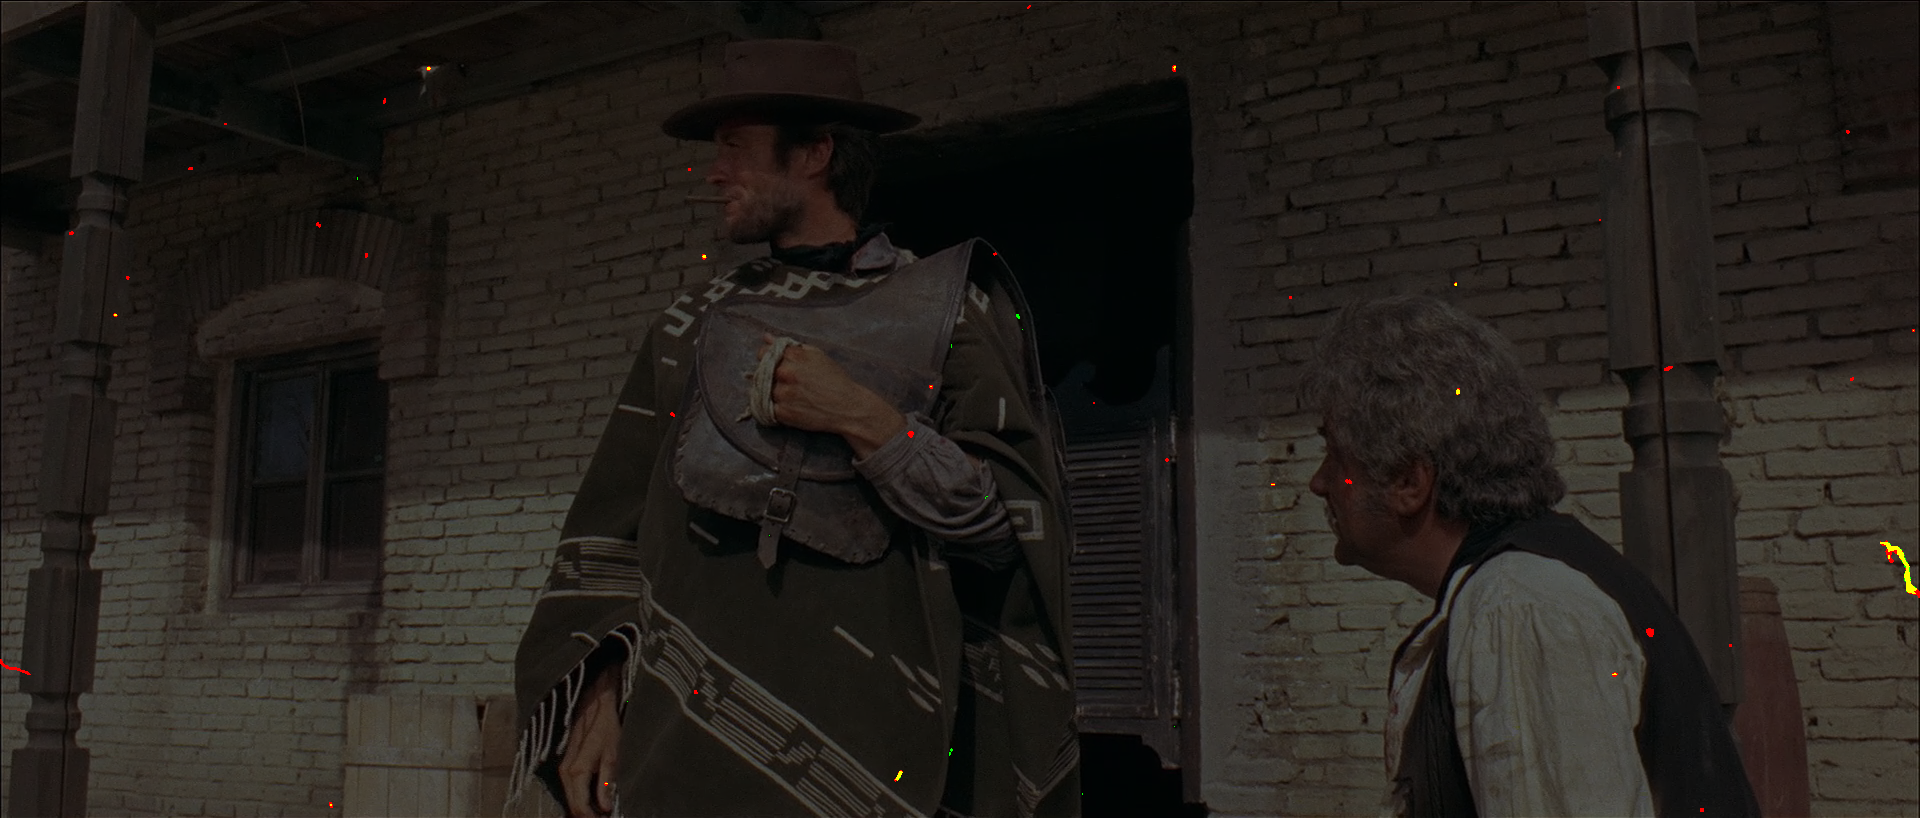
\includegraphics[width=0.7\linewidth]{images/punado_dollars_frame_0122-mask_big_dataset_r2attunetreduced_60_v1.png_comparaison.png}
	\caption{\smaller Inference result with the Fig. 8 image, using the baseline R2AttU-Net model with the new perfected dataset.} 
\end{figure}
As it can be seen in Fig. \ref{fig:11}, the dataset improvements have improved performance by a huge margin, practically removing the false positives detected in the first iteration. \\
On the next image, the one trained with the AttU-Net model we can see even better performance than the U-Net model, mostly on the dark regions of the image. Finally we can see that the worst model in this iteration of training is the R2AttU-Net model, missing a lot of the spots other models detect. 
\newpage
\subsubsection*{Pretraining}
Finally the pretrained model was trained. It was only tested the pretrained AttU-Net model, as the AttU-Net was found to be the best performing one yet. 
\begin{figure}[h!]
	\centering
	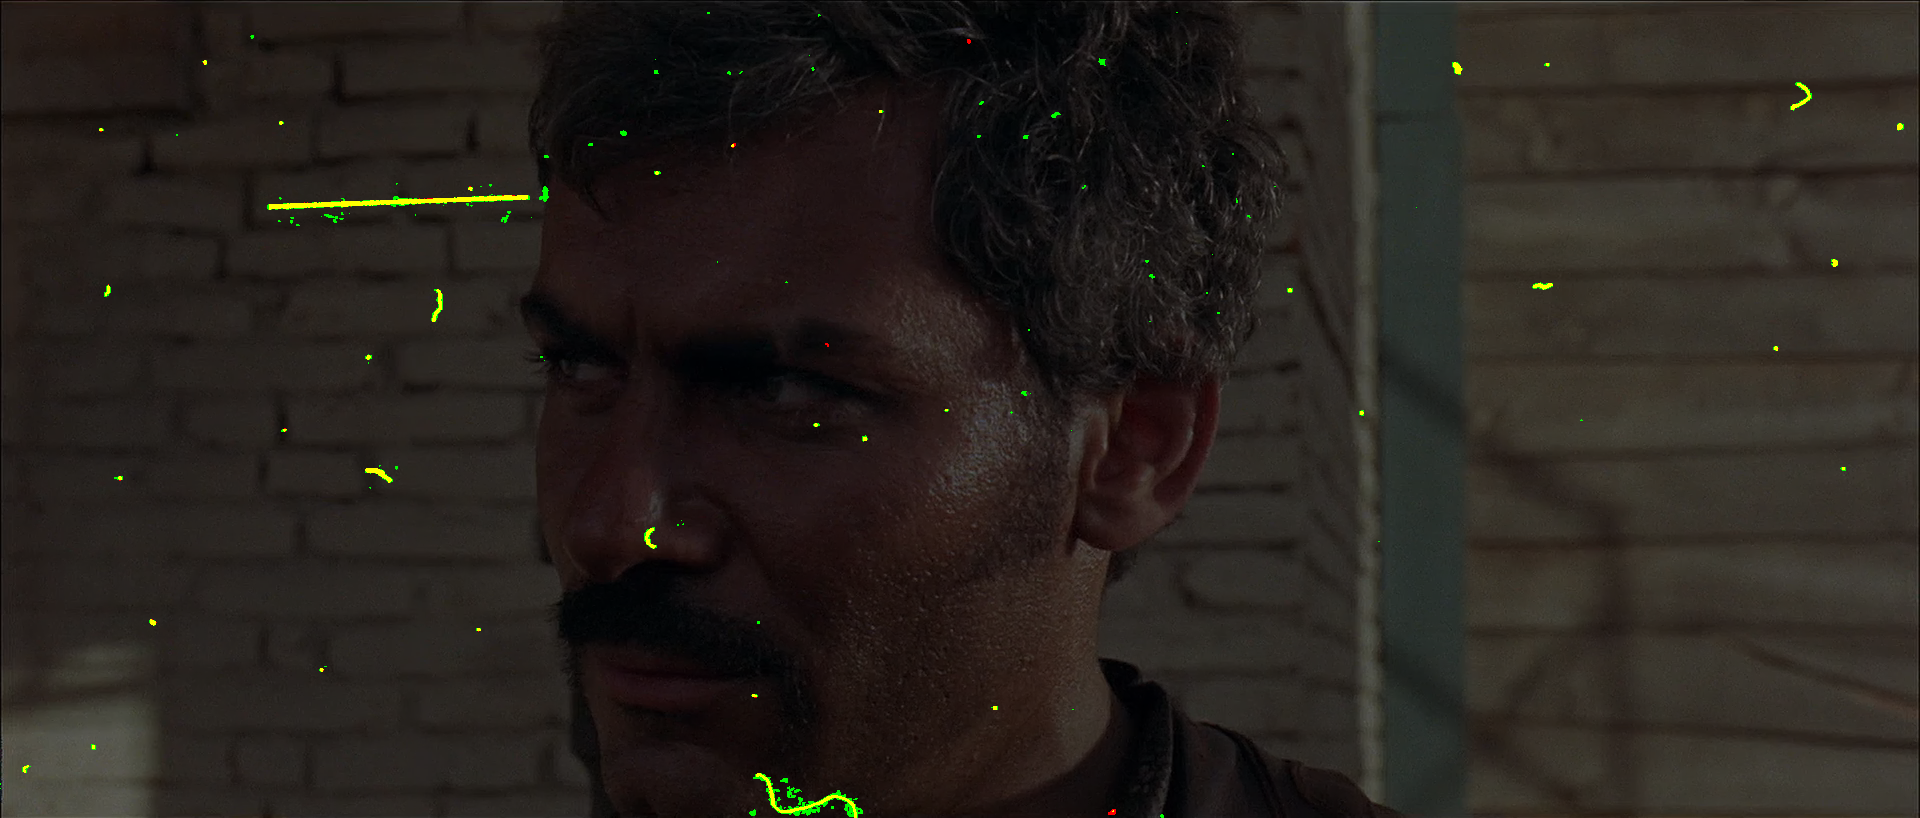
\includegraphics[width=0.7\linewidth]{images/punado_dollars_frame_0084-mask_pretrained_unet_40_epoch_oldloader_v1.png_comparaison.png}
	\caption{\smaller Inference result with the Fig. 7 image, using the baseline AttU-Net model with the perfected dataset.} 
	\label{fig:14}
\end{figure}
\begin{figure}[h!]
	\centering
	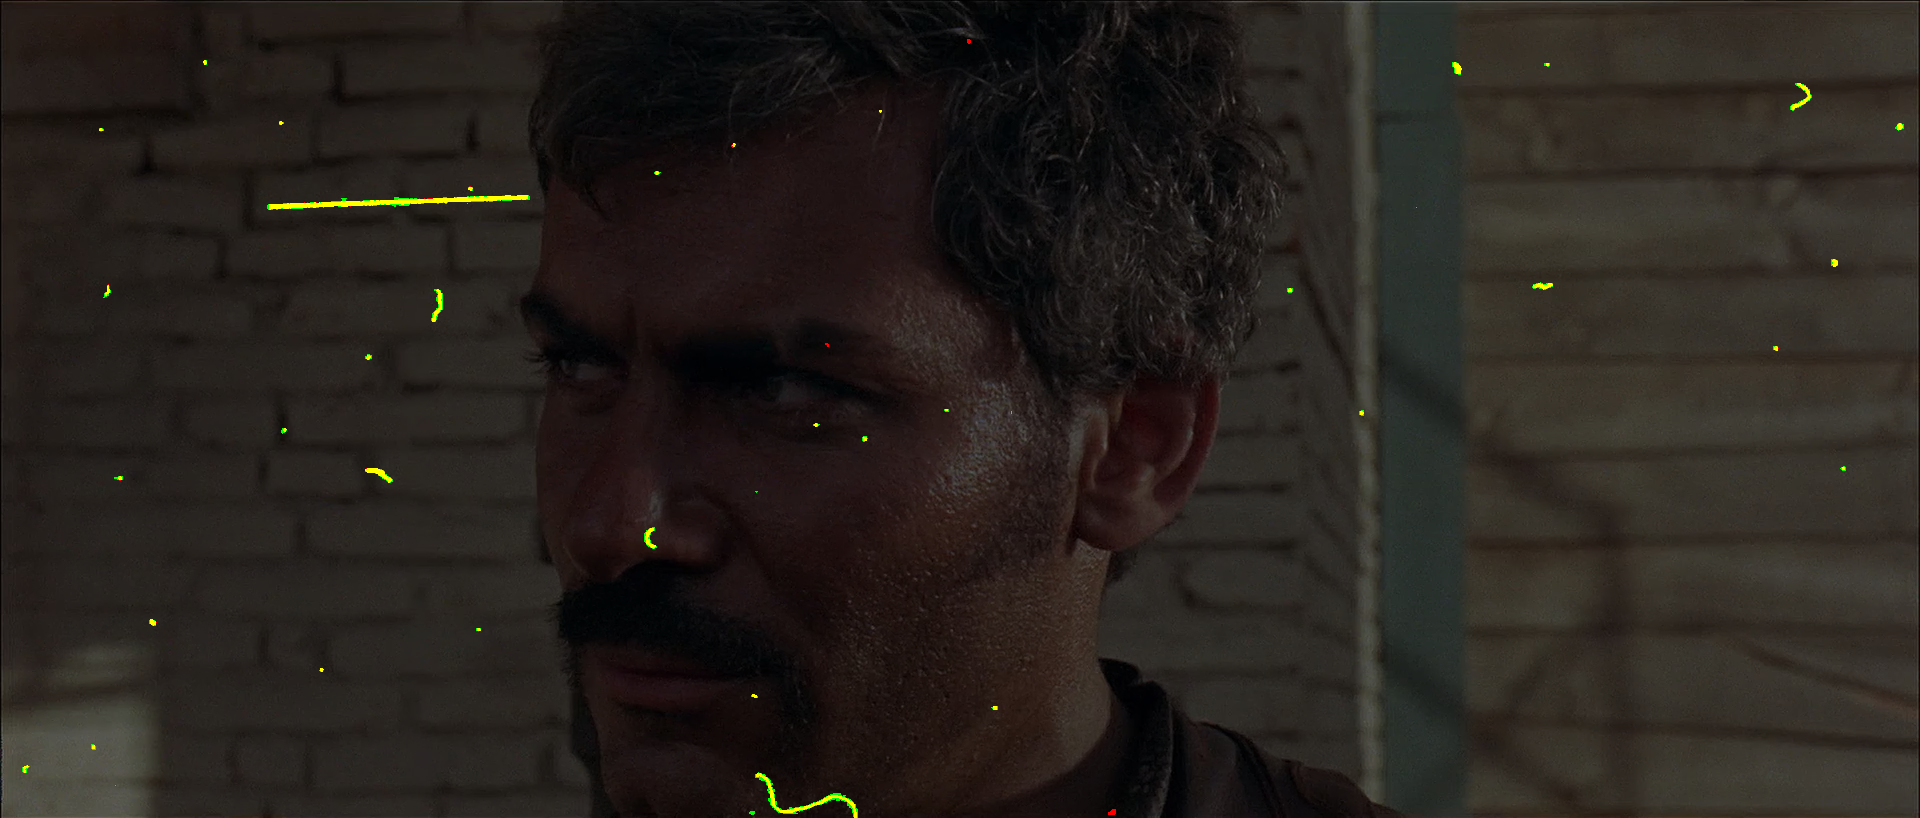
\includegraphics[width=0.7\linewidth]{images/punado_dollars_frame_0084-mask_big_dataset_unet_50_v1.png_comparaison.png}
	\caption{\smaller Inference result with the Fig. 7 image, using the pretrained AttU-Net model with the perfected dataset.} 
\end{figure}
As it can be observed mostly in the hair of the character, the baseline AttU-Net detects more false positives than the pretrained one. this can be observed across the test dataset. 
\subsection{Inpainting}
Unfortunately the current results for the RePaint experiments are poor in number. I've only generated a few examples, even though they are end to end (the mask has been detected with the segmentation model), and the diffusion model is still not a custom model but an already trained one, however the results are already acceptable in this stage of the project. Firstly I tried to run the RePaint inference just with the original mask generated by the segmentation. As it can be seen in the following side-by-side images, it did not change at all, the specs are still there. 
\begin{figure}[htbp]
	\centering
	\begin{minipage}{0.45\textwidth}
		\centering
		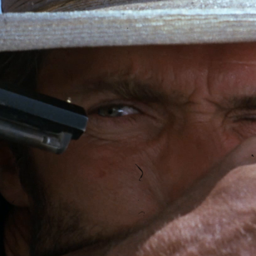
\includegraphics[width=\textwidth]{images/gt_image.png}
		\caption{Original dirty image. }
	\end{minipage}
	\hspace{0.05\textwidth}
	\begin{minipage}{0.45\textwidth}
		\centering
		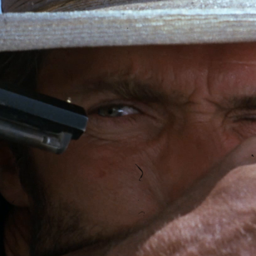
\includegraphics[width=\textwidth]{images/bueno_feo_malo_frame_0129_inpaint.png}
		\caption{Result of the RePaint generation}
	\end{minipage}
\end{figure}
To fix this, I tried to dilate the mask generated for a few pixels, as the results would not be much affected if it generated a bit more image than it should. As it can be seen in the next comparaisons, it worked perfectly.
\begin{figure}[htbp]
	\centering
	\begin{minipage}{0.45\textwidth}
		\centering
		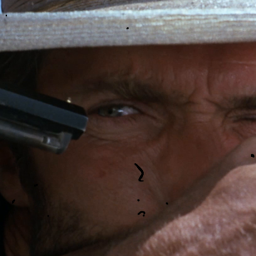
\includegraphics[width=\textwidth]{images/masked_3.png}
		\caption{\smaller Dirty image with dilated mask.}
	\end{minipage}
	\hspace{0.05\textwidth}
	\begin{minipage}{0.45\textwidth}
		\centering
		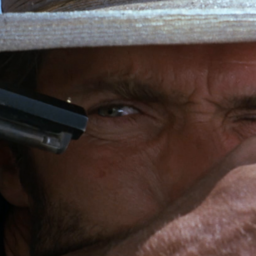
\includegraphics[width=\textwidth]{images/inpainted_3.png}
		\caption{Result of the RePaint generation}
	\end{minipage}
\end{figure}
\begin{figure}[htbp]
	\centering
	\begin{minipage}{0.45\textwidth}
		\centering
		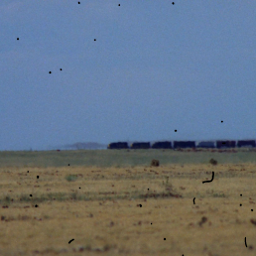
\includegraphics[width=\textwidth]{images/masked_2.png}
		\caption{\smaller Dirty image with dilated mask.}
	\end{minipage}
	\hspace{0.05\textwidth}
	\begin{minipage}{0.45\textwidth}
		\centering
		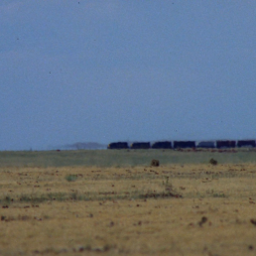
\includegraphics[width=\textwidth]{images/inpainted_2.png}
		\caption{Result of the RePaint generation}
	\end{minipage}
\end{figure}
\begin{figure}[htbp]
	\centering
	\begin{minipage}{0.45\textwidth}
		\centering
		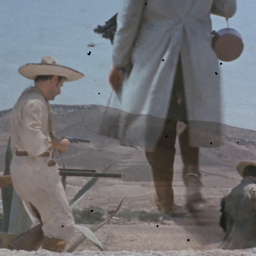
\includegraphics[width=\textwidth]{images/masked_4.png}
		\caption{\smaller Dirty image with dilated mask.}
	\end{minipage}
	\hspace{0.05\textwidth}
	\begin{minipage}{0.45\textwidth}
		\centering
		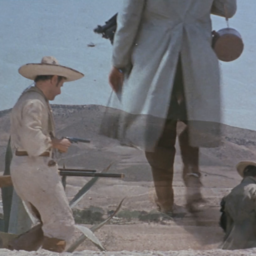
\includegraphics[width=\textwidth]{images/inpainted_4.png}
		\caption{Result of the RePaint generation}
	\end{minipage}
\end{figure}
\newpage
	\section{Final goal of the project}
Following the completion of this report, I have deemed it appropriate to revisit and refine the initial objectives of the project. The original aim centered on developing a viable solution to the posed problem. While the current pipeline represents significant progress toward this objective, it has yet to achieve optimal performance. Consequently, I have found it pertinent to explore an alternative methodological approach—one that diverges substantially from the present framework.\\
\\Specifically, I intend to investigate a unified diffusion-based architecture capable of addressing both the "segmentation" and inpainting tasks simultaneously. Although this novel approach does not explicitly perform segmentation in the conventional sense, it holds promise as a holistic solution that may streamline and potentially outperform traditional multi-stage pipelines. As this direction remains largely unexplored in the context of this project, it offers a compelling opportunity for comparative analysis and innovation.\\
\\
Moreover, a critical milestone for the next phase of the work will involve conducting a thorough evaluation of the metrics used to assess model performance. A comprehensive study of both quantitative and qualitative evaluation criteria will be essential in ensuring the reliability and consistency of the comparisons drawn between the different models. This step will not only strengthen the empirical foundation of the project but also provide a clearer perspective on the efficacy and limitations of each proposed approach.\clearpage
	\newpage
	\bibliography{references_initial}{}
	\nocite{kaji_overview_2019}
	\nocite{leejunhyun_leejunhyunimage_segmentation_2025}
	\nocite{zhu_denoising_2023}
	\nocite{xie_star_2025}
	\nocite{xie_segformer_2021}
	\bibliographystyle{plain}
	
	\end{document}
	
	
